%%%%%%%% ICML 2026 EXAMPLE LATEX SUBMISSION FILE %%%%%%%%%%%%%%%%%

\documentclass{article}

% Recommended, but optional, packages for figures and better typesetting:
\usepackage{microtype}
\usepackage{graphicx}
\usepackage{subcaption}
\usepackage{booktabs} % for professional tables
\usepackage{tikz}
\usepackage{svg}
\usepackage{algorithm2e}



% hyperref makes hyperlinks in the resulting PDF.
% If your build breaks (sometimes temporarily if a hyperlink spans a page)
% please comment out the following usepackage line and replace
% \usepackage{icml2026} with \usepackage[nohyperref]{icml2026} above.
\usepackage{hyperref}


% Attempt to make hyperref and algorithmic work together better:
\newcommand{\theHalgorithm}{\arabic{algorithm}}

% Use the following line for the initial blind version submitted for review:
\usepackage{icml2026}

% For preprint, use
% \usepackage[preprint]{icml2026}

% If accepted, instead use the following line for the camera-ready submission:
% \usepackage[accepted]{icml2026}

\usepackage{amsmath}
\usepackage{amssymb}
\usepackage{mathtools}
\usepackage{amsthm}


% if you use cleveref..
\usepackage[capitalize,noabbrev]{cleveref}

%%%%%%%%%%%%%%%%%%%%%%%%%%%%%%%%
% THEOREMS
%%%%%%%%%%%%%%%%%%%%%%%%%%%%%%%%
\theoremstyle{plain}
\newtheorem{theorem}{Theorem}[section]
\newtheorem{proposition}[theorem]{Proposition}
\newtheorem{lemma}[theorem]{Lemma}
\newtheorem{corollary}[theorem]{Corollary}
\theoremstyle{definition}
\newtheorem{definition}[theorem]{Definition}
\newtheorem{assumption}[theorem]{Assumption}
\theoremstyle{remark}
\newtheorem{remark}[theorem]{Remark}

% Todonotes is useful during development; simply uncomment the next line
%    and comment out the line below the next line to turn off comments
%\usepackage[disable,textsize=tiny]{todonotes}
\usepackage[textsize=tiny]{todonotes}

% The \icmltitle you define below is probably too long as a header.
% Therefore, a short form for the running title is supplied here:
\icmltitlerunning{Limits of RL for decision tree policies}

\begin{document}

\twocolumn[
  \icmltitle{Limits of reinforcement learning for decision trees in\\ Markov decision processes}

  % It is OKAY to include author information, even for blind submissions: the
  % style file will automatically remove it for you unless you've provided
  % the [accepted] option to the icml2026 package.

  % List of affiliations: The first argument should be a (short) identifier you
  % will use later to specify author affiliations Academic affiliations
  % should list Department, University, City, Region, Country Industry
  % affiliations should list Company, City, Region, Country

  % You can specify symbols, otherwise they are numbered in order. Ideally, you
  % should not use this facility. Affiliations will be numbered in order of
  % appearance and this is the preferred way.
  \icmlsetsymbol{equal}{*}

  \begin{icmlauthorlist}
    \icmlauthor{Hector Kohler}{yyy, sch}
    \icmlauthor{Riad Akrour}{comp, sch}
    \icmlauthor{Philippe Preux}{comp, sch}
    %\icmlauthor{}{sch}
    %\icmlauthor{}{sch}
  \end{icmlauthorlist}

  \icmlaffiliation{yyy}{Laboratiore d'Informatique, \'Ecole Polytechnique, Paris, France}
  \icmlaffiliation{comp}{CRIStAL, Universit\'e de Lille, Lille, France}
  \icmlaffiliation{sch}{Inria, France}

  \icmlcorrespondingauthor{Hector Kohler}{hector.kohler@polytechnique.edu}

  % You may provide any keywords that you find helpful for describing your
  % paper; these are used to populate the "keywords" metadata in the PDF but
  % will not be shown in the document
  \icmlkeywords{Reinforcement learning, decision trees, POMDP}

  \vskip 0.3in
]

% this must go after the closing bracket ] following \twocolumn[ ...

% This command actually creates the footnote in the first column listing the
% affiliations and the copyright notice. The command takes one argument, which
% is text to display at the start of the footnote. The \icmlEqualContribution
% command is standard text for equal contribution. Remove it (just {}) if you
% do not need this facility.

% Use ONE of the following lines. DO NOT remove the command.
% If you have no special notice, KEEP empty braces:
\printAffiliationsAndNotice{}  % no special notice (required even if empty)
% Or, if applicable, use the standard equal contribution text:
% \printAffiliationsAndNotice{\icmlEqualContribution}

\begin{abstract}
  For applications like medicine where model interpretability is critical, decision trees might be preferred over neural networks because humans can read their predictions from the root to the leaves.
%   Learning decision trees for classification or regression problems is well understood: there exists many supervised learning algorithms that return decision trees optimizing some trade-off of interpretability and performances.
%   Comparatively, learning such decision trees for sequential decision making problems is a new research direction.
  Most of the litterature on interpretable reinforcement learning that focuses on imitating (or distilling) neural networks.
  In contrast, we study reinforcement learning algorithms returning decision trees that optimize some trade-off of cumulative rewards and interpretability in a Markov decision process (MDP). 
  We show that such algorithms can be seen as learning policies for partially observable Markov decision processes (POMDPs).
  We use this parallel to understand why in practice it is often easier to use imitation learning than to learn the decision tree from scratch for sequential decision making problems.
\end{abstract}

\section{Introduction}
Interpretable machine learning provides either local or global interpretations \cite{glanois-survey}.
Global methods, like decision tree induction~\cite{breiman1984classification}, return a model whose outputs can be interpreted without having to run an additional algorithm.
By contrast, local methods require to run an additional algorithm, e.g. linear regression~\cite{regression}, but are agnostic to the model class.

Local interpretable model-agnostic explanations (LIME)~\cite{lime} is a popular local interpretability method.
Given a model, LIME works by perturbing the input and learning a simple interpretable model locally to explain that particular prediction (cf. figure~\ref{fig:lime}). 
For each individual prediction, LIME provides interpretations by identifying which features were most important for that specific decision.

Local interpretability can also be called explainability.
Global interpretability methods constrain the model class so that the computations are transparent or verifiable by construction. 
On the other hand, explainability methods--or local interpretability methods--keep black-box models and generates post hoc explanations of their decisions. 
In additions to linear models, explanations can take various forms: visual explanations with saliency maps \cite{Puri2020Explain}, attribution such as SHAP\cite{shap}, attention-based highlighting \cite{attention}.

While useful for insight, these explanations are often subjective and might not be faithful to the underlying computations~\cite{Atrey2020Exploratory}.
For safety-critical settings, this motivates our focus on models that are interpretable by design.
Those interpretable by design models can be obtained by global interpretability methods that we present next.

\begin{figure*}
    \centering
    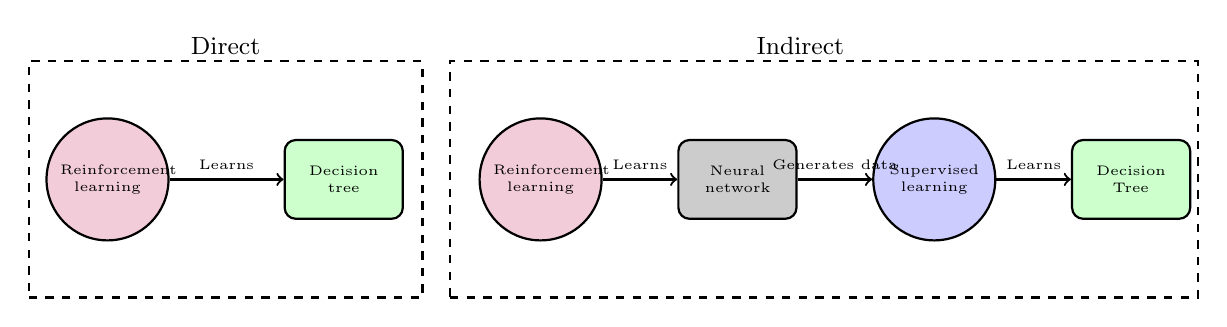
\begin{tikzpicture}[
        node distance=2cm,
        auto,
        thick,
        rl/.style={circle, draw, fill=purple!20, minimum width=1.5cm, minimum height=0.8cm, text centered},
        nn/.style={rectangle, draw, fill=black!20, rounded corners, minimum width=1.5cm, minimum height=1cm, text centered},
        sl/.style={circle, draw, fill=blue!20, minimum width=1.5cm, minimum height=0.8cm, text centered},
        dt/.style={rectangle, draw, fill=green!20, rounded corners, minimum width=1.5cm, minimum height=1cm, text centered},
        arrow/.style={->, thick},
        label/.style={font=\tiny, above},
        method_box/.style={rectangle, draw, dashed, minimum width=5cm, minimum height=3cm, text centered},
        method_box_indirect/.style={rectangle, draw, dashed, minimum width=9.5cm, minimum height=3cm, text centered}
    ]
        
        % Direct method box
        \node[method_box] (direct_box) at (-0.5,0) {};
        \node at (-0.5,1.7) {\small{Direct}};
        
        % Direct method - RL process
        \node[rl] (rl_direct) at (-2,0) {
            \begin{minipage}{1.2cm}
                \centering
                % \includesvg[width=0.3cm]{images/images_intro/gear-file-svgrepo-com.svg}\\
                \tiny{Reinforcement learning}
            \end{minipage}
        };
        
        % Direct method - Decision Tree
        \node[dt] (dt_direct) at (1,0) {
            \begin{minipage}{1.2cm}
                \centering
                % \includesvg[width=0.3cm]{images/images_intro/decision-tree-svgrepo-com.svg}\\
                \tiny{Decision tree}
            \end{minipage}
        };
        
        % Direct method arrow
        \draw[arrow] (rl_direct) -- (dt_direct) node[label, midway] {\tiny Learns};
        
        % Indirect method box
        \node[method_box_indirect] (indirect_box) at (7.1,0) {};
        \node at (6.8,1.7) {\small{Indirect}};
        
        % Indirect method - RL process
        \node[rl] (rl_indirect) at (3.5,0) {
            \begin{minipage}{1.2cm}
                \centering
                % \includesvg[width=0.3cm]{images/images_intro/gear-file-svgrepo-com.svg}\\
                \tiny{Reinforcement learning}
            \end{minipage}
        };
        
        % Indirect method - Neural Network
        \node[nn] (nn_indirect) at (6,0) {
            \begin{minipage}{1.2cm}
                \centering
                % \includesvg[width=0.3cm]{images/images_intro/network-mapping-svgrepo-com.svg}\\
                \tiny{Neural network}
            \end{minipage}
        };
        
        % Indirect method - Supervised Learning
        \node[sl] (sl_indirect) at (8.5,0) {
            \begin{minipage}{1.2cm}
                \centering
                % \includesvg[width=0.3cm]{images/images_intro/gear-file-svgrepo-com.svg}\\
                \tiny{Supervised learning}
            \end{minipage}
        };
        
        % Indirect method - Decision Tree
        \node[dt] (dt_indirect) at (11,0) {
            \begin{minipage}{1.2cm}
                \centering
                % \includesvg[width=0.3cm]{images/images_intro/decision-tree-svgrepo-com.svg}\\
                \tiny{Decision Tree}
            \end{minipage}
        };
        
        % Indirect method arrows
        \draw[arrow] (rl_indirect) -- (nn_indirect) node[label, midway] {\tiny Learns};
        \draw[arrow] (nn_indirect) -- (sl_indirect) node[label, midway] {\tiny Generates data};
        \draw[arrow] (sl_indirect) -- (dt_indirect) node[label, midway] {\tiny Learns};
        
    \end{tikzpicture}
    \caption{Comparison of direct and indirect approaches for learning interpretable models in sequential decision making.}
    \label{fig:direct-vs-indirect-methods}
\end{figure*}

Global approaches are either direct or indirect~\cite{milani-survey}. 
Direct algorithms, such as decision tree induction~\cite{breiman1984classification}, \textit{directly} learn an interpretable model optimizing some objective (cf. figure~\ref{fig:interpretability-performance-tradeoff}).
One key challenge motivating this work is that decision tree induction is well-developed for supervised learning but not for reinforcement learning.
To directly learn interpretable models for sequential decision making, one must design new algorithms which will be the core of this paper. 

Most existing research has focused on developing indirect methods. 
Indirect methods for interpretable sequential decision making—sometimes called \textit{post hoc} methods—begin by learning a non-interpretable model (e.g., reinforcement learning of a neural network model), and then use supervised learning to fit an interpretable model that emulates the black-box.
Indirect methods rely on behavior cloning or imitation learning~\cite{behavior-cloning,dagger} to emulate the black-box models.
Most work on interpretable sequential decision focuses on the indirect approach\cite{viper,PIRL}.

Verifiable Reinforcement learning via Policy Extraction, or VIPER \cite{viper}, is a strong indirect method to learn decision tree models for sequential decision making. VIPER first trains a neural network model with reinforcement learning and then fit a decision tree to minimize the disagreement between the neural network and the tree outputs given the same inputs.
They show that decision tree models, in addition to being transparent, are also fast to verify in the formal sense of the term \cite{maraboupy}.
Programmatic models are an interpretable class that contains decision trees. 
Programmatically Interpretable Reinforcement Learning (PIRL) \cite{PIRL} synthesizes programs in a domain-specific language, also by imitating a neural network model. 

However, unlike direct methods that return interpretable models optimizing the desired objective, indirect methods learn an interpretable model to match the behavior of a black-box that itself optimizes the objective of interest. 
Due to the restricted policy class, the best decision tree model might employ a completely different strategy than the best black-box neural network model to solve the task.
Furthermore, the decision tree model that best fits the best neural network model might be sub-optimal compared to the decision tree model that best solves the task of interest.
Hence, there is no guarantee that optimizing this surrogate objective of best emulating a black-box yields the best interpretability–performance trade-offs. 
Figure~\ref{fig:direct-vs-indirect-methods} illustrates the key difference between these two approaches. 

Beyond direct and indirect learning, a complementary strategy is to train experts that are inherently easier to imitate and understand.
This is achieved by adding interpretability-oriented regularization during training. In the context of supervised learning tasks, the authors of \cite{parbhoo} regularize the neural network model during training such that indirect approaches will be biased towards more interpretable trees.

In addition to finding models which computations can be read by humans or that can be formally verified, interpretable machine learning has also been used to detect reward misalignment in sequential decision making: by exposing the decision process of a model, one can identify goal mis-specification or unintended shortcuts.
Such shortcuts can be, for example, following the shadow of someone instead of actually following someone because for the model they lead to the same reactions.
The learning of interpretable models for misalignment detection has been heavily studied by Quentin Delfosse contemporarily to this manuscript \cite{scobots,shindo2024blendrl,nudge,ocatari}.

\subsection{Contributions}
We show that direct reinforcement learning of decision tree policies for MDPs (cf. definition~\ref{def:mdp}), i.e. learning a decision tree that optimizes the RL objective (cf. definition~\ref{def:mdp-obj}) is often very difficult.
In particular, we provide some insights as to why it is so difficult and show that indirect imitation of a neural network policy (cf. section \ref{sec:imit}), despite optimizing the imitation learning objective (cf. definition~\ref{def:il}) rather than the RL one, often yields very good tree policies in practice.

This first part of the manuscript is organized as follows.
In this chapter, we present Nicholay Topin and colleagues' framework for direct reinforcement learning of decision tree policies~\cite{topin2021iterative}.
In chapter \ref{sec:topin}, we reproduce experiments from~\cite{topin2021iterative} where we compare direct deep reinforcement learning (cf. section \ref{sec:drl}) of decision tree policies to indirect imitation of neural network policies with decision trees for the simple CartPole MDP~\cite{cartpole}.
In chapter \ref{sec:pomdp}, we show that this direct approach is equivalent to learning a deterministic memoryless policy for partially observable MDP (POMDP)\cite{POMDP,chap2}--which is a hard problem~\cite{littman1}--and show that this might be the main reason for failures.
In chapter \ref{sec:pomdp-classif}, we further support this claim by constructing special instances of such POMDPs where the observations contain all the information about hidden states, and show that in those cases, direct reinforcement learning of decision trees works well.  

\section{Learning decision tree policies for MDPs}\label{related-work-pomdp}
In the introductory example (cf. section~\ref{sec:limits-il}), we have shown that imitation learning algorithms that optimize the imitation learning objective (cf. definition~\ref{def:il}) rather than the RL objective, are, unsurprisingly, prone to sub-optimality w.r.t. the latter objective.
This motivates the study and development of \textit{direct} decision tree policy learning algorithms.
There already exists such algorithms that return decision tree policies optimizing the RL objective for a given MDP.
Those algorithms either learn parametric trees or non-parametric trees.

Parametric trees are not ``grown'' from the root by iteratively adding internal or leaf nodes (cf. figure~\ref{fig:dt}), but are rather ``optimized'': the depth, internal nodes arrangement, and state features to consider in each node are fixed \textit{a priori} and only the thresholds of each node are learned.
This is similar to doing gradient descent on neural network weights.
As the reader might have guessed, those parametric trees are advantageous in that they can be learned with the policy gradient \cite{pg_sutton}.
In \cite{silva},~\cite{vos2024optimizinginterpretabledecisiontree} and~\cite{sympol}, the authors use PPO (cf. algorithm~\ref{alg:ppo}) to learn such differentiable decision trees that optimize directly the RL objective.
In particular, \cite{sympol} explicitly studies the gap in RL objective values between their direct optimization and the imitation learning algorithm VIPER (cf. algorithm~\ref{alg:viper}).
While those methods return decision tree policies that optimize the RL objective well, in general a user cannot know \textit{a priori}  what a ``good'' tree policy structure should be for a particular MDP.
It could be that the specified structure is too deep and pruning will be required after training or it could be that the tree structure is not expressive enough to encode a good policy, i.e. parametric trees cannot trade off interpretability and performances during training.
Furthermore, the authors from~\cite{sympol} show that extra stabilizing tricks, such as adaptive batch sizes, are required during training to outperform indirect imitation in terms of RL objective.

Non-parametric trees are the standard model in supervised learning. Greedy algorithms~\cite{breiman1984classification,ID3,c45} are fast and return decision tree classifiers (or regressors) that offer good trade-offs between interpretability (depth, or number of nodes) and the supervised learning objective (cf. definition~\ref{def:sl}).
On the other hand, to the best of our knowledge, there exists only one work studying non-parametric trees to optimize a trade-off between interpretability and the RL objective: Topin et. al. \cite{topin2021iterative}.

Given an MDP for which one wants to learn a decision tree policy, Topin et. al. introduced iterative bounding Markov decision processes (IBMDPs).
From now on we refer to the MDP for which we want a decision tree policy as the ``base'' MDP.
IBMDPs are an augmented version of this base MDP with more state features, more actions, additional reward signals, and additional transitions.
Authors showed that certain policies in IBMDPs are equivalent to non-parametric decision tree policies that trade off between interpretability and the RL objective in the base MDP.
Hence, the great promise of Topin et. al.'s work is that doing e.g. RL to learn such IBMDP policies is a way to directly optimize a trade-off between interpretability and the RL objective.

There also exists more specialized approaches that can return decision tree policies only for very specific problem classes.
In \cite{theory1}, the authors prove that for maze-like MDPs, there always exists an optimal decision tree policy w.r.t. the RL objective and provide an algorithm to find it. 
Finally, in \cite{dt-opt-mdp}, the authors study decision tree policies for planning in MDPs (cf. algorithm~\ref{alg:value-iteration}), i.e. when the transitions and rewards are known.

\section{Technical preliminaries}
\subsection{What are decision trees?}
As the reader might have already guessed, we will put great emphasis on decision tree models as a means to study interpretability.
While other interpretable models might have other properties than the ones we will highlight through this thesis, one conjecture from \cite{glanois-survey} is that interpretable models are all hard to optimize or learn because they are non-differentiable in nature.
This is something that will be key in our study of decision tree models that we introduce next and that we illustrate in figure~\ref{fig:dt}.

\begin{definition}[Decision tree]\label{def:dt}
    A decision tree is a rooted tree $T = (\mathcal{N}, E)$.
    Each internal node $\nu \in \mathcal{N}$ is associated with a test that maps input features $x_{ij} \in \mathcal{X}$ to a Boolean.
    Each edge $e \in E$ from an internal node corresponds to an outcome of the associated test function.
    Each leaf node $l \in \mathcal{N}$ is associated with a prediction $y_l \in \mathcal{Y}$, where $\mathcal{Y}$ is the output space.
    For any input $x \in \mathcal{X}$, the tree defines a unique path from root to leaf, determining the prediction $T(x) = y_l$ where $l$ is the reached leaf.
    The depth of a tree is the maximum path length from root to any leaf.
\end{definition}

\begin{figure}
    \centering
    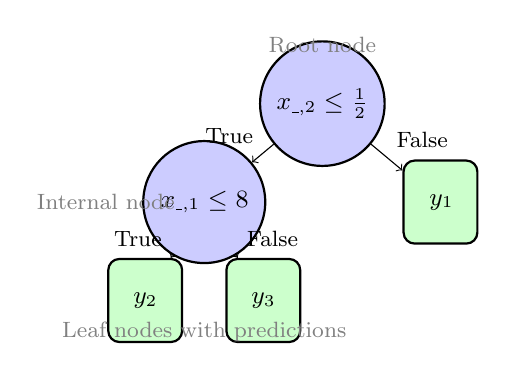
\begin{tikzpicture}[
        scale=0.5,
        decision/.style={circle, draw, thick, fill=blue!20, text width=3.5em, text centered, minimum height=3.5em, font=\small},
        leaf/.style={rectangle, draw, thick, fill=green!20, text width=2em, text centered, rounded corners, minimum height=3em, font=\small},
        edge_label/.style={font=\footnotesize, midway}
    ]
        % Root decision node
        \node[decision] (root) at (0,0) {$x_{\_, 2} \leq \frac{1}{2}$};
        
        % Second level nodes
        \node[decision] (left_decision) at (-3, -2.5) {$x_{\_, 1}\leq 8$};
        \node[leaf] (right_leaf) at (3, -2.5) {$y_1$};
        
        % Third level nodes (leaves)
        \node[leaf] (left_left) at (-4.5, -5) {$y_2$};
        \node[leaf] (left_right) at (-1.5, -5) {$y_3$};
        
        % Connections with labels
        \draw[->] (root) -- (left_decision) node[edge_label, above left] {True};
        \draw[->] (root) -- (right_leaf) node[edge_label, above right] {False};
        \draw[->] (left_decision) -- (left_left) node[edge_label, above left] {True};
        \draw[->] (left_decision) -- (left_right) node[edge_label, above right] {False};
        
        % Add labels for components
        \node[font=\footnotesize, text=gray] at (0, 1.5) {Root node};
        \node[font=\footnotesize, text=gray] at (-5.5, -2.5) {Internal node};
        \node[font=\footnotesize, text=gray] at (-3, -5.8) {Leaf nodes with predictions};
        
    \end{tikzpicture}
    \caption{A generic depth 2 decision tree with 2 nodes and 3 leaves. The root node applies the test $1_{\{x_{\_,1}\leq \frac{1}{2}\}}$ to check if the first features of data is below $\frac{1}{2}$. Edges represent the outcomes of the tests in each internal nodes(True/False), and leaf nodes contain predictions $y_l \in \mathcal{Y}$. For any input $\boldsymbol{x}_i$, the tree defines a unique path from root to leaf.}
    \label{fig:dt}
\end{figure}

\subsection{Markov decision processes and problems}

Markov decision processes (MDPs) were first introduced in the 1950s by Richard Bellman~\cite{Bellman}.
Informally, an MDP models how an agent acts over time to achieve a goal. 
At every time step, the agent observes its current state (e.g., patient weight and tumor size) and takes an action (e.g., administers a certain amount of chemotherapy).
The agent receives a reward that helps evaluate the quality of the action with respect to the goal (e.g., tumor size decreases when the objective is to cure cancer).
Finally, the agent transitions to a new state (e.g., the updated patient state) and repeats this process over time. 
Following Martin L. Puterman's book on MDPs\cite{puterman}, we formally define:
\begin{definition}[Markov decision process]\label{def:mdp} An MDP is a tuple $\mathcal{M} = \langle S, A, R, T, T_0 \rangle$ where:
\begin{itemize}
\item $S$ is a finite set of states representing all possible configurations of the environment.
\item $A$ is a finite set of actions available to the agent.
\item $R: S \times A \rightarrow \mathbb{R}$ is a deterministic reward function that assigns a real-valued reward to each state-action pair. While in general reward functions are often stochastic, in this manuscript we focus deterministic ones without loss of generality.
\item $T: S \times A \rightarrow \Delta(S)$ is the transition function that maps state-action pairs to probability distributions over next states $\Delta(S)$.
\item $T_0 \in \Delta(S)$ is the initial distribution over states.
\end{itemize}
\end{definition}

Informally, we would like to act in an MDP so that we obtain as much reward as possible over time.
For example, in cancer treatment, the best outcome is to eliminate the patient's tumor as quickly as possible.
We can formally define this objective, that we call the reinforcement learning objective, as follows:

\begin{definition}[Reinforcement learning objective]\label{def:mdp-obj} Given an MDP $\mathcal{M}\equiv\langle S, A, R, T, T_0 \rangle$ (cf. definition~\ref{def:mdp}), the goal of reinforcement learning for sequential decision making is to find a model, also known as a policy, $\pi: S \rightarrow A$ that maximizes the expected discounted sum of rewards:
$$J(\pi) = \mathbb{E}\left[\sum_{t=0}^{\infty} \gamma^t R(s_t, a_t) \mid s_0 \sim T_0, a_t = \pi(s_t), s_{t+1} \sim T(s_t, a_t)\right]$$
where $0< \gamma\leq 1$ is the discount factor that controls the trade-off between immediate and future rewards.
\end{definition}

Algorithms presented in this manuscript aim to find an optimal policy $\pi^\star \in\underset{\pi}{\operatorname{argmax}}J(\pi)$ that maximizes the above reinforcement learning (RL) objective.

\subsection{Example: a grid world MDP}
\begin{figure}
    \centering
    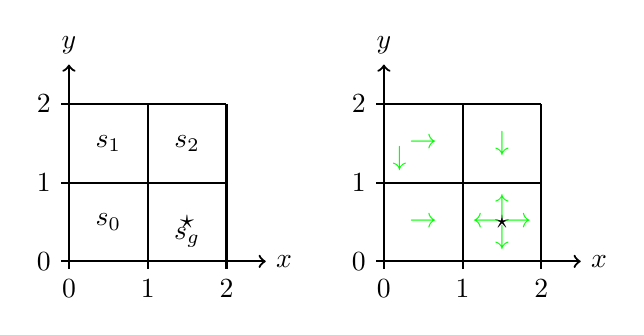
\begin{tikzpicture}
        \tikzstyle{grid}=[draw, thick, fill=gray!10]
        
        % Draw grid
        \draw[grid] (0,0) grid (2,2);
        
        % Add axes
        \draw[thick, ->] (0,0) -- (2.5,0) node[right] {$x$};
        \draw[thick, ->] (0,0) -- (0,2.5) node[above] {$y$};
        
        % Add tick marks and labels
        \foreach \x in {0,1,2} {
            \draw[thick] (\x,0) -- (\x,-0.1) node[below] {$\x$};
        }
        \foreach \y in {0,1,2} {
            \draw[thick] (0,\y) -- (-0.1,\y) node[left] {$\y$};
        }
        
        % Add state labels clockwise from bottom left
        \node at (0.5,0.5) {$s_0$};
        \node at (1.5,0.5) {$\star$};
        \node at (1.5,0.3) {$s_g$};
        \node at (1.5,1.5) {$s_2$};
        \node at (0.5,1.5) {$s_1$};


        % Draw grid
        \draw[grid] (4,0) grid (6,2);
        
        % Add axes
        \draw[thick, ->] (4,0) -- (6.5,0) node[right] {$x$};
        \draw[thick, ->] (4,0) -- (4,2.5) node[above] {$y$};
        
        % Add tick marks and labels
        \draw[thick] (4,0) -- (4,-0.1) node[below] {$0$};
        \draw[thick] (5,0) -- (5,-0.1) node[below] {$1$};
        \draw[thick] (6,0) -- (6,-0.1) node[below] {$2$};
        

        \foreach \y in {0,1,2} {
            \draw[thick] (4,\y) -- (3.9,\y) node[left] {$\y$};
        }
        
        % Add state labels clockwise from bottom left
        \node at (4.5,0.5) {{\color{green} $\rightarrow$}};
        \node at (5.5,0.5) {$\star$};
        \node at (5.5,0.7) {{\color{green} $\uparrow$}};
        \node at (5.5,0.3) {{\color{green} $\downarrow$}};
        \node at (5.7,0.5) {{\color{green} $\rightarrow$}};
        \node at (5.3,0.5) {{\color{green} $\leftarrow$}};
        \node at (5.5,1.5) {{\color{green} $\downarrow$}};
        \node at (4.2,1.3) {{\color{green} $\downarrow$}};
        \node at (4.5,1.5) {{\color{green} $\rightarrow$}};
    \end{tikzpicture}
    \caption{A grid world MDP (left) and optimal actions w.r.t. the objective (cf. definition~\ref{def:mdp-obj}) (right).}\label{example:grid}
    \end{figure}

In figure~\ref{example:grid}, we present a very simple MDP (cf. definition~\ref{def:mdp}).
This MDP is essentially a grid where the starting state is chosen at random and the goal is to reach the bottom-right cell as fast as possible in order to maximize the RL objective (cf. definition~\ref{def:mdp-obj}).
The state space is discrete with state labels representing 2D-coordinates.
The actions are to move up, left, right, or down. 
The bottom-right cell gives reward 1 and is an absorbing state, i.e., once in the state, the MDP stays in this state forever.
Other states give reward 0 and are not absorbing.
The optimal actions that get to the goal as fast as possible in every state (cell) are presented in green in figure~\ref{example:grid}.
Next we present the tools to find solutions to MDPs and compute such optimal policies.

\section{Exact solutions for Markov decision problems}\label{sec:values}
We begin with the planning setting in which the MDP transitions and rewards (cf. definition~\ref{def:mdp}) are known. 
Leveraging the Markov property, one can use dynamic programming~\cite{Bellman} to compute optimal policies with respect to the RL objective (cf. definition~\ref{def:mdp-obj}).
Algorithms based on dynamic programming use the notion of \textit{value} of states and actions:
\begin{definition}[Value of a state]\label{def:vs} 
    In an MDP $\mathcal{M}$ (cf. definition~\ref{def:mdp}), the value of a state $s\in S$ under policy $\pi$ is the expected discounted sum of rewards starting from state $s$ and following policy $\pi$:
    $$V^\pi(s) = \mathbb{E}\left[\sum_{t=0}^{\infty} \gamma^t R(s_t, a_t) \mid s_0 = s, a_t = \pi(s_t), s_{t+1} \sim T(s_t, a_t)\right]$$
    Applying the Markov property gives a recursive definition of the value of $s$ under policy $\pi$:
    $$V^\pi(s) = R(s,\pi(s)) + \gamma \mathbb{E}\left[V^\pi(s') | s'\sim T(s, \pi(s))\right]$$
\end{definition}
\begin{definition}[Optimal value of a state] The optimal value of a state $s\in S$, $V^\star(s)$, is the value of state $s$ when following the optimal policy $\pi^{\star}$ (the policy that maximizes the RL objective (cf. definition~\ref{def:mdp-obj})).
    $$V^{\star}(s) = V^{\pi^{\star}}(s)$$
\end{definition}
\begin{definition}[Optimal value of a state–action pair]\label{def:qvalues} The optimal value of a state–action pair $(s,a)\in S\times A$, $Q^\star(s,a)$, is the value when taking action $a$ in state $s$ and then following the optimal policy.
    $$Q^{\star}(s,a) = R(s, a) + \gamma\mathbb{E}\left[V^{\star}(s') | s'\sim T(s, a)\right]$$
\end{definition}

More realistically, neither the transition function $T$ nor the reward function $R$ of the MDP are known, e.g. the doctor cannot \textbf{know} how the tumor and the patient's health will change after a dose of chemotherapy, but can only \textbf{observe} the change.
This distinction in available information parallels the distinction between dynamic programming and reinforcement learning, described next. 

\subsection{Reinforcement learning of approximate solutions to MDPs}\label{sec:rl}
When the MDP transition function and reward function are unknown, one can use reinforcement learning algorithms--also known as agents--to learn values or policies maximizing the RL objective. 
Reinforcement learning algorithms popularized by Richard Sutton~\cite{sutton} don't \textbf{compute} an optimal policy but rather \textbf{learn} an approximate one based on sequences of transitions $(s_t, a_t, r_t, s_{t+1})_t$.
RL algorithms usually fall into two categories: value-based~\cite{sutton} and policy search~\cite{pg_sutton}.
Examples of these approaches are shown in algorithms~\ref{alg:qlearning},~\ref{alg:sarsa} and~\ref{alg:reinforce}.
Q-learning and Sarsa compute an approximation of $Q^{\star}$ (cf. definition~\ref{def:qvalues}) using temporal difference learning~\cite{sutton}. Q-learning is \textit{off-policy}: it collects new transitions with a random policy, e.g. epsilon-greedy. Sarsa is \textit{on-policy}: it collects new transitions greedily w.r.t. the current Q-values estimates.
Policy gradient algorithms~\cite{pg_sutton} leverage the policy gradient theorem to approximate $\pi^{\star}$.

Q-learning, Sarsa, and policy gradients algorithms are known to converge to the optimal value or (locally) optimal policy under some conditions.
There are many other ways to learn policies such as simple random search~\cite{random-search} or model-based reinforcement learning that estimates MDP transitions and rewards before applying e.g. value iteration~\cite{ucbvi}. 
Those RL algorithms--also known as tabular RL because they represent policies as tables with $|S|\times |A|$ entries--are limited to small state spaces.
To scale to large state spaces, it is common to use a neural network to represent policies or values~\cite{tdgammon}.
In the next section, we present deep reinforcement learning algorithms designed specifically for neural networks.
\RestyleAlgo{ruled}
\SetKwComment{Comment}{}{}
\begin{algorithm}
    \KwData{MDP $\mathcal{M} = \langle S, A, R, T, T_0 \rangle$, learning rate $\alpha$, exploration rate $\epsilon$}
    \KwResult{Policy $\pi$}
    Initialize $Q(s,a) = 0$ for all $s \in S, a \in A$ \\
    Initialize state $s_0 \sim T_0$ \\
    \For{each step $t$}{
        Choose action $a_t$ using e.g. $\epsilon$-greedy policy: $a_t = \operatorname{argmax}_a Q(s_t,a)$ with prob. $1-\epsilon$ \\
        Take action $a_t$, observe $r_t = R(s_t,a_t)$ and $s_{t+1} \sim T(s_t,a_t)$ \\
        $Q(s_t,a_t) \leftarrow Q(s_t,a_t) + \alpha[r_t + \gamma \max_{a'} Q(s_{t+1},a') - Q(s_t,a_t)]$ \\
        $s_t \leftarrow s_{t+1}$ \\
    }
    $\pi(s) = \operatorname{argmax}_a Q(s,a)$ \Comment{// Extract greedy policy}
    \caption{Q-Learning~\cite{watkins1992q}}\label{alg:qlearning}
\end{algorithm}

\subsection{Deep reinforcement learning}
Reinforcement learning has also been successfully combined with function approximations to solve MDPs with large discrete state spaces or continuous state spaces ($S\subset \mathbb{R}^p$ in definition~\ref{def:mdp}).
In the rest of this manuscript, unless stated otherwise, we write $\boldsymbol{s}$ a state vector in a continuous state space\footnote{Note that discrete states can be one-hot encoded as state vectors in $\{0, 1\}^{|S|}$.}.

Deep Q-Networks (DQN)~\cite{dqn}, described in algorithm~\ref{alg:dqn} achieved super-human performance on a set of Atari games.
Authors successfully extended the Q-learning (cf. algorithm~\ref{alg:qlearning}) to the function approximation setting by introducing target networks to mitigate distributional shift in the temporal difference error and replay buffer to increase sample efficiency.

Proximal Policy Optimization (PPO)~\cite{ppo}, described in algorithm~\ref{alg:ppo}, is an actor-critic algorithm~\cite{sutton} optimizing a neural network policy. 
In actor-critic algorithms, cumulative discounted rewards starting from a particular state, also known as \textit{the returns}, are also estimated with a neural network. 
PPO is known to work well in a variety of domains including robot control in simulation among others.


\subsection{Imitation learning: a baseline (indirect) interpretable reinforcement learning method}\label{sec:imit}

Unlike PPO or DQN for neural networks, there exists no algorithm that trains decision tree policies to optimize the RL objective (cf. definition~\ref{def:mdp-obj}).
In fact, we will show in the first part of the manuscript that training decision trees that optimize the RL objective is very difficult.

Hence, many interpretable reinforcement learning approaches first train a neural network policy--also called an expert policy--to optimize the RL objective (cf. definition~\ref{def:mdp-obj}) using e.g. PPO, and then fit a student policy such as a decision tree using CART (cf. algorithm~\ref{alg:cart}) to optimize the supervised learning objective (cf. definition~\ref{def:sl}) with the neural policy actions as targets.
This approach is known as imitation learning and is essentially training a student policy to optimize the objective:

\begin{definition}[Imitation learning objective]\label{def:il}
Given an MDP $\mathcal{M}$ (cf. definition~\ref{def:mdp}), an expert policy $\pi^*$ and a policy class $\Pi$, e.g. decision trees of depth at most 3, the imitation learning objective is to find a student policy $\hat{\pi} \in \Pi$ that minimizes the expected action disagreement with the expert:
\begin{equation}
IL(\pi) = \mathbb{E}_{\boldsymbol{s} \sim \rho(\boldsymbol{s})} \left[ \mathcal{L}(\pi(\boldsymbol{s}), \pi^*(\boldsymbol{s})) \right]
\end{equation}
where $\rho(\boldsymbol{s})$ is the state distribution in $\mathcal{M}$ induced by the student policy $\pi$ and $\mathcal{L}$ is a loss function measuring the disagreement between the student policy's action $\pi(s)$ and the expert's action $\pi^*(s)$.
\end{definition}

There are two main imitation learning methods used for interpretable reinforcement learning.
Dagger (cf. algorithm~\ref{alg:dagger}) is a straightforward way to fit a decision tree policy to optimize the imitation learning objective (cf. definition~\ref{def:il}).
VIPER (cf. algorithm~\ref{alg:viper}) was designed specifically for interpretable reinforcement learning.
VIPER re-weights the transitions collected by the neural network expert by a function of the state-action value (cf. definition~\ref{sec:values}).
The authors of VIPER showed that decision tree policies fitted with VIPER tend to have the same RL objective value as Dagger trees while being more interpretable (shallower or with fewer nodes) and sometimes outperform Dagger trees.
Dagger and VIPER are two strong baselines for decision tree learning in MDPs, but they optimize a surrogate objective only, even though in practice the resulting decision tree policies often achieve high RL objective value.
We use these two algorithms extensively throughout the manuscript.
Next we show how to learn a decision tree policy for the example MDP (cf. figure~\ref{example:grid}).

\subsection{Your first decision tree policy}\label{sec:limits-il}
Now the reader should know how to train decision tree classifiers or regressors for supervised learning using CART (cf. section~\ref{sec:sl}).
The reader should also know what an MDP is and how to compute or learn policies that optimize the RL objective (cf. definition~\ref{def:mdp-obj}) with (deep) reinforcement learning (cf. section~\ref{sec:drl}).
Finally, the reader should now know how to obtain a decision tree policy for an MDP through imitation learning (cf. definition~\ref{def:il}) by first using RL to get an expert policy and then fitting a decision tree to optimize the supervised learning objective, using the expert actions as labels.

In this section we present the first decision tree policies of this manuscript obtained using Dagger or VIPER after learning an expert Q-function for the grid world MDP from figure~\ref{example:grid} using Q-learning (cf. algorithm~\ref{alg:qlearning}).
Recall the optimal policies for the grid world, taking the green actions in each state in figure~\ref{example:grid}. 
Among the optimal policies, the ones that go left or up in the goal state can be problematic for imitation learning algorithms.
Indeed, we know that for this grid world MDP there exists decision tree policies with a very good interpretability-performance trade-off: depth-1 decision trees that are optimal w.r.t. the RL objective.
One could even say that those trees have the \textit{optimal} interpretability-performance trade-off because they are the shortest trees that are optimal w.r.t. the RL objective.

In figure~\ref{fig:trees-intro}, we present a depth-1 decision tree policy that is optimal w.r.t. the RL objective and a depth-1 tree that is sub-optimal.
The other optimal depth-1 tree is to go right when $y\leq 1$ and down otherwise.
Indeed, figure~\ref{fig:objectives} shows that the optimal depth-1 tree achieves exactly the same RL objective value as the optimal policies from figure~\ref{example:grid}, independently of the discount factor $\gamma$.

Now a fair question is: can Dagger or VIPER learn such an optimal depth-1 tree given access to an expert optimal policy from figure~\ref{example:grid}?

We start by running the standard Q-learning algorithm as presented in algorithm~\ref{alg:qlearning} with $\epsilon=0.3$, $\alpha=0.1$ over 10,000 time steps.
The careful reader might wonder how ties are broken in the $\operatorname{argmax}$ operation from algorithm~\ref{alg:qlearning}.
While Sutton and Barto break ties by index value in their book~\cite{sutton} (the greedy action is the $\operatorname{argmax}$ action with smallest index), we show that the choice of tie-breaking greatly influences the performance of subsequent imitation learning algorithms.
Indeed, depending on how actions are ordered in practice, Q-learning may be biased toward some optimal policies rather than others.
While this does not matter for one who just wants to find an optimal policy, in our example of finding the optimal depth-1 decision tree policy, it matters \textit{a lot}.

In the left plot of figure~\ref{fig:ql-il}, we see that Q-learning, independently of how ties are broken, consistently converges to an optimal policy over 100 runs (random seeds).
However, in the right plot of figure~\ref{fig:ql-il}, where we plot the proportion over 100 runs of optimal decision trees returned by Dagger or VIPER at different stages of Q-learning, we observe that imitating the optimal policy obtained by breaking ties at random consistently yields more optimal trees than breaking ties by indices.
What actually happens is that the most likely output of Q-learning when ties are broken by indices is the optimal policy that goes left in the goal state,
which cannot be perfectly represented by a depth-1 decision tree, because there are three different actions taken and a binary tree of depth $D=1$ can only map to $2^D=2$ labels.

This short experiment shows that imitation learning approaches can sometimes be very bad at learning decision tree policies with good interpretability-performance trade-offs for very simple MDPs. 
Despite VIPER almost always finding the optimal depth-1 decision tree policy in terms of the RL objective when ties are broken at random, we have shed light on the sub-optimality of indirect approaches such as imitation learning.
This motivates the study of direct approaches (cf. figure~\ref{fig:direct-vs-indirect-methods}) to directly search for policies with good interpretability-performance trade-offs with respect to the original RL objective.

\begin{figure}
    \centering
    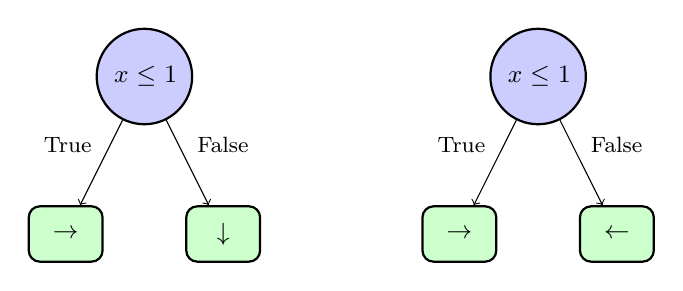
\begin{tikzpicture}[
        decision/.style={circle, draw, thick, fill=blue!20, text width=2.5em, text centered, minimum height=2.5em, font=\small},
        leaf/.style={rectangle, draw, thick, fill=green!20, text width=2em, text centered, rounded corners, minimum height=2em, font=\small},
        edge_label/.style={font=\footnotesize, midway}
    ]
        % Tree 4: if x <= 0.5 move right else move left
        \node[decision] (tree4_root) at (10,2) {$x \leq 1$};
        \node[leaf] (tree4_right) at (9,0) {$\rightarrow$};
        \node[leaf] (tree4_left) at (11,0) {$\leftarrow$};
        \draw[->] (tree4_root) -- (tree4_right) node[edge_label, above left] {True};
        \draw[->] (tree4_root) -- (tree4_left) node[edge_label, above right] {False};
        \tikzstyle{grid}=[draw, thick, fill=gray!10]


        % Tree 4: if x <= 0.5 move right else move left
        \node[decision] (tree5_root) at (5,2) {$x \leq 1$};
        \node[leaf] (tree5_right) at (4,0) {$\rightarrow$};
        \node[leaf] (tree5_left) at (6,0) {$\downarrow$};
        \draw[->] (tree5_root) -- (tree5_right) node[edge_label, above left] {True};
        \draw[->] (tree5_root) -- (tree5_left) node[edge_label, above right] {False};
        \tikzstyle{grid}=[draw, thick, fill=gray!10]

    \end{tikzpicture}
    \caption{Left, an optimal depth-1 decision tree policy. On the right, a sub-optimal depth-1 decision tree policy.}\label{fig:trees-intro}
    \end{figure}

\begin{figure*}
    \centering
    \includegraphics[width=1\textwidth]{../images/images_part1/base_mdp.pdf}
    \caption{Left, sample complexity curve of Q-learning with default hyperparameters on the $2\times 2$ grid world MDP over 100 random seeds. Right, performance of indirect interpretable methods when imitating the greedy policy with a tree at different Q-learning stages.}\label{fig:ql-il}
\end{figure*}

\section{Iterative bounding Markov decision processes}\label{sec:ibmdp}

The key thing to know about IBMDPs is that they are, as their name suggests, MDPs (cf definition~\ref{def:mdp}).
Hence, IBMDPs admit an optimal deterministic Markovian policy that maximizes the RL objective.
In this part we will assume that all the MDPs we consider are MDPs with continuous state spaces (cf. section~\ref{sec:drl}) with a finite set of actions, so we use bold fonts for states and observations as they are vector-valued.
However all our results generalize to discrete states (in $\mathbb{Z}^m$) MDPs that we can factor using one-hot encodings. 
Given an MDP for which we want to learn a decision tree policy--the base MDP--IBMDP states are concatenations of the base MDP state features and some observations. 
Those observations are information about the base state features that are refined--``iteratively bounded''-- at each step.
Those observations essentially represent some knowledge about where some base state features lie in the state space.
Actions available in an IBMDP are: 1) the actions of the base MDP, that change base state features, and 2) \textit{information gathering} actions that change the aforementioned observations.
Now, base actions in an IBMDP are rewarded like in the base MDP, this ensures that the RL objective w.r.t. the base MDP is encoded in the IBMDP reward.
When taking an information gathering action, the reward is an arbitrary value such that optimizing the RL objective in the IBMDP is equivalent to optimizing some trade-off between interpretability and the RL objective in the base MDP.
 
Before showing how to get decision tree policies from IBMDP policies, we give a formal definition of IBMDPs following Topin et. al.~\cite{topin2021iterative}.

\begin{definition}[Iterative bounding Markov decision process]\label{def:ibmdp}
Given an MDP $\mathcal{M}\equiv\langle S, A, R, T, T_0 \rangle$ (cf. definition~\ref{def:mdp}), an associated iterative bounding Markov decision process $\mathcal{M}_{IB}$ is a tuple:
\begin{align*}
    \langle \overbrace{S \times O}^{\text{State space}}, \underbrace{A \cup A_{info}}_{\text{Action space}}, \overbrace{(R, \zeta)}^{\text{Reward function}}, \underbrace{(T_{info}, T, T_0)}_{\text{Transitions}}\rangle
\end{align*}
, where: 
\begin{itemize}
\item $S$ are the base MDP state features. Base state features $\boldsymbol{s} = (s_1, \dots, s_p)\in S$ are bounded: $s_j \in [L_j, U_j]$ where $\infty < L_j \leq U_j < \infty \forall 1\leq j \leq p$.
\item $O$ are observations. They represent bounds on the base state features: $O\subsetneq S^2 =  [L_1, U_1]\times \dots \times [L_p, U_p] \times [L_1, U_1]\times \dots \times [L_p, U_p]$. So the complete IBMDP state space is $S \times O$, the concatenations of base state features and observations
Given some base state features $\boldsymbol{s} = (s_1, \dots, s_p)\in S$ and some observation $\boldsymbol{o} = (L_1, U_1, \dots, L_p, U_p)$, an IBMDP state is $\boldsymbol{s}_{IB} = (\overbrace{s_1, \dots, s_p}^{\text{base state features}}, \underbrace{L_1, U_1, \dots, L_p, U_p}_{\text{observation}})$.
\item $A$ are the base MDP actions.
\item $A_{info}$ are \textit{information gathering} actions (IGAs) of the form $\langle j, v \rangle$ where $j$ is a state feature index $1 \leq j \leq p$ and $v$ is a real number between $L_j$ and $U_j$. So the complete action space of an IBMDP is the set of base MDP actions and information gathering actions $A \cup A_{info}$.
\item $R: S\times A \rightarrow \mathbb{R}$ is the base MDP reward function.
\item $\zeta$ is a reward signal for taking an information gathering action.
So the IBMDP reward function is to get a reward from the base MDP if the action is a base MDP action or to get $\zeta$ if the action is an IGA action.
\item $T_{info}: S\times O \times( A_{info} \cup A )\rightarrow \Delta (S\times O)$ is the transition function of IBMDPs: 
Given some observation $\boldsymbol{o}_t = (L'_1, U'_1, \dots, L'_p, U'_p) \in O$ and base state features $\boldsymbol{s}_t=(s'_1, s'_2, \dots, s'_p)$ if an IGA $\langle j, v \rangle$ is taken, the new observation is:
\begin{align*}
    \boldsymbol{o}_{t+1} &= \begin{cases}
        (L'_1, U'_1, \dots , L'_j, \min\{v, U'_j\}, \dots , L''_p, U'_p) \text{ if } s_j \leq v\\
        (L'_1, U'_1, \dots , \max\{v, L'_j\}, U'_j, \dots , L''_p, U'_p) \text{ if } s_j > v
    \end{cases}
\end{align*}
If a base action is taken, the observation is reset to the default base state feature bounds $(L_1, U_1,\dots, L_p, U_p)$ and the base state features change according to the base MDP transition function: $\boldsymbol{s}_{t+1}\sim T(\boldsymbol{s}_t, a_t)$.
At initialization, the base state features are drawn from the base MDP initial distribution $T_0$ and the observation is always set to the default base state features bounds $\boldsymbol{o}_0=(L_1, U_1,\dots, L_p, U_p)$.
\end{itemize}
\end{definition}

Now remains to extract a decision tree policy for MDP $\mathcal{M}$ from a policy for an associated IBMDP $\mathcal{M}_{IB}$. 

\subsection{From policies to trees}

One can notice that information gathering actions (cf. definition~\ref{def:ibmdp}) resemble the Boolean functions $1_{\{x_{\_, j} \leq v\}}$ that make up internal decision tree nodes (cf. figure~\ref{fig:dt}).
Indeed, a policy taking actions in an IBMDP essentially builds a tree by taking sequences of IGAs (internal nodes) and then a base action (leaf node) and repeats this process over time.
In particular, the IGA rewards $\zeta$ can be seen as a regularization or a penalty for interpretability: if $\zeta$ is very small compared to base rewards, a policy will try to take base actions as often as possible, i.e. build shallow trees with short paths between root and leaves.

Authors from~\cite{topin2021iterative} show that not all IBMDP policies are decision tree policies for the base MDP.
In particular, they show that only deterministic policies depending solely on the observations of the IBMDP are guaranteed to correspond to decision tree policies for the base MDP.

\begin{proposition}[Deterministic partially observable IBMDP policies are decision tree policies]\label{def:po-policy}
    Given a base MDP $\mathcal{M}$ $\langle S, A, R, T, T_0\rangle$ and an associated IBMDP $\mathcal{M}_{IB}$ $\langle S \times O,A \cup A_{info}, (R, \zeta), (T_{info}, T, T_0)\rangle$ (cf. definition~\ref{def:ibmdp}), a deterministic partially observable policy $\pi_{po}: O \rightarrow A\cup A_{info}$ is a decision tree policy $\pi_{\mathcal{T}}: S \rightarrow A$ for the base MDP $\mathcal{M}$.
\end{proposition}

\begin{proof}(Sketch) algorithm~\ref{alg:extract-tree} that takes as input a deterministic partially observable policy (cf. definition~\ref{def:po-policy}) for an IBMDP $\mathcal{M}_{IB}$ $\langle S \times O,A \cup A_{info}, (R, \zeta), (T_{info}, T, T_0)\rangle$ (cf. definition~\ref{def:ibmdp}), returns a decision tree policy $\pi_{\mathcal{T}}$ (cf. definition~\ref{sec:dt}) for the base MDP $\mathcal{M}$ $\langle S, A, R, T, T_0\rangle$ and always terminates unless the deterministic partially observable policy takes IGAs in every state.
\end{proof}

\begin{algorithm}[t]
    \KwData{Deterministic partially observable policy $\pi_{po}$ for IBMDP $ \langle S \times O,A \cup A_{info}, (R, \zeta), (T_{info}, T, T_0)\rangle$ and IBMDP observation $\boldsymbol{o}=(L'_1, U'_1, \dots, L'_p, U'_p)$}
    \KwResult{Decision tree policy $\pi_{\mathcal{T}}$ for MDP $\langle S, A, R, T, T_0\rangle$}
    
    \SetKwProg{Fn}{Function}{:}{}
    \SetKwFunction{SubtreeFromPolicy}{Subtree\_From\_Policy}
    
    \Fn{\SubtreeFromPolicy{$\boldsymbol{o}, \pi_{po}$}}{
        $a \leftarrow \pi_{po}(\boldsymbol{o})$ \\
        \If{$a$ is a base action}{
            \Return Leaf\_Node(action: $a$) \Comment{// Leaf if base action}
        }
        \Else{
            $\langle i, v\rangle \leftarrow a$ \Comment{// Splitting action is feature and value} \\
            $\boldsymbol{o}_L \leftarrow \boldsymbol{o}; \quad \boldsymbol{o}_R \leftarrow \boldsymbol{o}$ \\
                         $\boldsymbol{o}_L \leftarrow (L'_1, U'_1, \dots, L'_j, v, \dots, L'_p, U'_p); \quad \boldsymbol{o}_R \leftarrow (L'_1, U'_1, \dots, v, U'_j, \dots, L'_p, U'_p)$ \\
            $child_L \leftarrow$ Subtree\_From\_Policy$(\boldsymbol{o}_L, \pi_{po})$ \\
            $child_R \leftarrow$ Subtree\_From\_Policy$(\boldsymbol{o}_R, \pi_{po})$ \\
            \Return Internal\_Node(feature: $i$, value: $v$, children: $(child_L, child_R)$)
        }
    }
    \caption{Extract a Decision Tree Policy}\label{alg:extract-tree}
\end{algorithm}

While the connections with partially observable MDPs~\cite{POMDP,chap2} is obvious, we defer the implications to chapter \ref{sec:pomdp} as this connection was absent from the original IBMDP paper~\cite{topin2021iterative}.
Next we present an IBMDP for the MDP of example~\ref{example:grid}.

\subsection{Example: an IBMDP for a grid world}
We re-formulate the example MDP (example~\ref{example:grid}) as an MDP with a finite number of vector valued states ($x,y$-coordinates).
The states are $S = \{(0.5, 0.5), (0.5, 1.5), (1.5, 1.5),$ $(1.5, 0.5)\}\subsetneq [0, 2] \times [0, 2]$.
The actions are the cardinal directions $A = \{\rightarrow, \leftarrow, \downarrow, \uparrow\}$ that shift the states by one as long as the coordinates remain in the grid.
The reward for taking any action is 0 except when in the bottom right state $(1.5, 0.5)$ which is an absorbing state: once in this state, you stay there forever. 
Standard optimal deterministic Markovian policies were presented for this MDP in example \ref{example:grid}.

Suppose an associated IBMDP (definition \ref{def:ibmdp}) with two IGAs:
\begin{itemize}
    \item $\langle x, 1\rangle$ that tests if $x\leq 1$
    \item $\langle y, 1\rangle$ that tests if $y\leq 1$
\end{itemize}
The initial observation is always the grid bounds $\boldsymbol{o}_0=(0, 2, 0, 2)$ because the base state features in the grid world are always in $[0, 2] \times [0, 2]$.
There are only finitely many observations since with those two IGAs there are only nine possible observations that can be attained from $\boldsymbol{o}_0$ following the IBMDP transitions (cf. definition \ref{def:ibmdp}).
For example when the IBMDP initial base state features are $\boldsymbol{s}_0 = (0.5, 1.5)$, and taking first $\langle x, 1\rangle$ then $\langle y, 1\rangle$ the corresponding observations are first $\boldsymbol{o}_{t+1} = (0, 1, 0, 2)$ and then $\boldsymbol{o}_{t+2} = (0, 1, 1, 2)$.
The full observation set is $O = \{(0, 2, 0, 2)$, $(0, 1, 0, 2)$, $(0, 2, 0, 1)$, $(0, 1, 0, 1)$, $(1, 2, 0, 2)$, $(1, 2, 0, 1)$, $(1, 2, 1, 2)$, $(0, 1, 1, 2)$, $(0, 2, 1, 2)\}$.
The transitions and rewards are given in definition (cf. definition~\ref{def:ibmdp}).

In figure~\ref{example:ibmdp} we illustrate a trajectory in this IBMDP.
\begin{figure*}
\centering
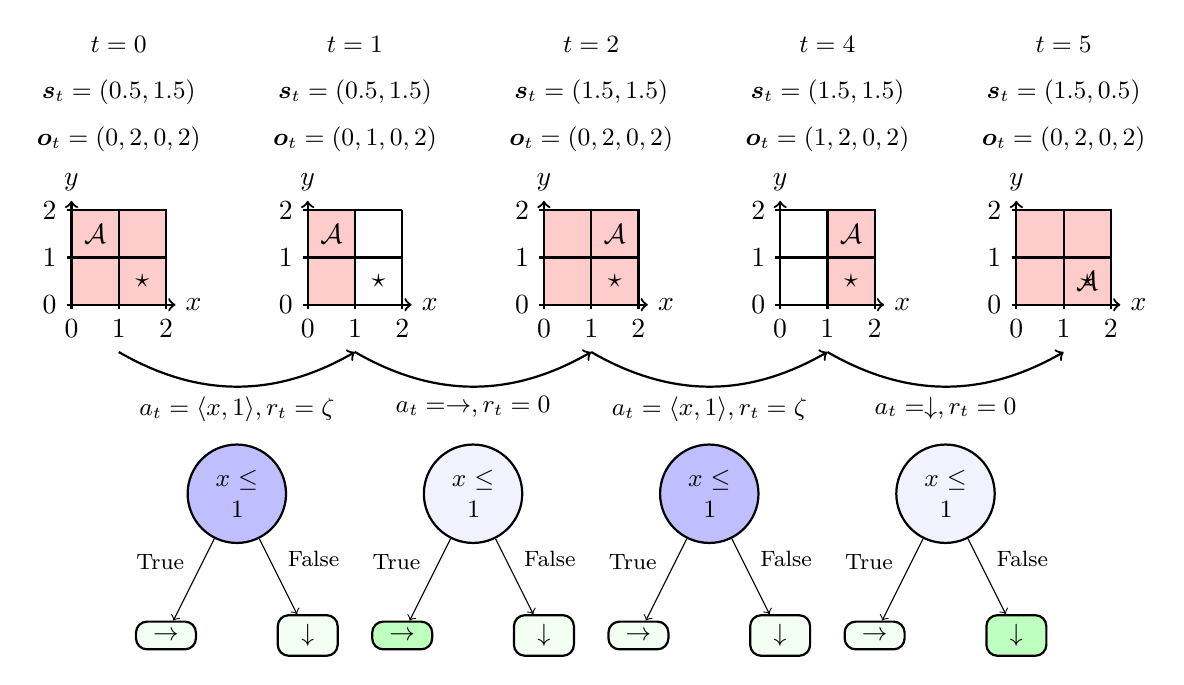
\begin{tikzpicture}[scale=0.6]
    % Define styles
    \tikzstyle{grid}=[draw, thick, fill=gray!10]
    \tikzstyle{rectangle}=[draw, thick, fill=red!20]
    
    % Row 1: IBMDP States (s, o)
    % t=0: Initial state
    \node at (2,9.5) {\small $t=0$};
    \node at (2,8.5) {\small $\boldsymbol{s}_t=(0.5, 1.5)$};
    \node at (2,7.5) {\small $\boldsymbol{o}_t=(0, 2, 0, 2)$};

    \draw[rectangle] (1,4) rectangle (3,6);
    \draw[grid] (1,4) grid (3,6);
    % Add axes
    \draw[thick, ->] (1,4) -- (3.2,4) node[right] {$x$};
    \draw[thick, ->] (1,4) -- (1,6.2) node[above] {$y$};
    \foreach \x in {0,1,2} {
        \draw[thick] (\x+1,4) -- (\x+1,3.9) node[below] {$\x$};
    }
    \foreach \y in {0,1,2} {
        \draw[thick] (1,\y+4) -- (0.9,\y+4) node[left] {$\y$};
    }
    \node at (1.5, 5.5) {$\mathcal{A}$};
    \node at (2.5, 4.5) {$\star$};
    
    % Curved arrow from t=0 to t=1
    \draw[thick, ->] (2,3) to[bend right=30] node[midway, below] {\small $a_t = \langle x, 1\rangle, r_t = \zeta$} (7,3);

    % % t=1: After AIG x≤0.5
    \node at (7,9.5) {\small $t=1$};
    \node at (7,8.5) {\small $\boldsymbol{s}_t=(0.5, 1.5)$};
    \node at (7,7.5) {\small $\boldsymbol{o}_t=(0, 1, 0, 2)$};

    \draw[rectangle] (6,4) rectangle (7,6);
    \draw[grid] (6,4) grid (8,6);
    % Add axes
    \draw[thick, ->] (6,4) -- (8.2,4) node[right] {$x$};
    \draw[thick, ->] (6,4) -- (6,6.2) node[above] {$y$};
    \foreach \x in {0,1,2} {
        \draw[thick] (\x+6,4) -- (\x+6,3.9) node[below] {$\x$};
    }
    \foreach \y in {0,1,2} {
        \draw[thick] (6,\y+4) -- (5.9,\y+4) node[left] {$\y$};
    }
    \node at (6.5, 5.5) {$\mathcal{A}$};
    \node at (7.5, 4.5) {$\star$};


    % Curved arrow from t=1 to t=2
    \draw[thick, ->] (7,3) to[bend right=30] node[midway, below] {\small $a_t = \rightarrow, r_t  = 0$}(12,3);

    \node[circle, draw, thick, fill=blue!25, text width=2em, text centered, minimum height=1.5em, font=\small] (tree4_root) at (4.5,0) {$x \leq 1$};
    \node[rectangle, draw, thick, fill=green!5, text width=1.5em, text centered, rounded corners, minimum height=1em, font=\small] (tree4_right) at (3,-3) {$\rightarrow$};
    \node[rectangle, draw, thick, fill=green!5, text width=1.5em, text centered, rounded corners, minimum height=1em, font=\small] (tree4_left) at (6,-3) {$\downarrow$};
    \draw[->] (tree4_root) -- (tree4_right) node[font=\footnotesize, midway, above left] {True};
    \draw[->] (tree4_root) -- (tree4_left) node[font=\footnotesize, midway, above right] {False};

    \node at (12,9.5) {\small $t=2$};
    \node at (12,8.5) {\small $\boldsymbol{s}_t=(1.5, 1.5)$};
    \node at (12,7.5) {\small $\boldsymbol{o}_t=(0, 2, 0, 2)$};
    
    \draw[rectangle] (11,4) rectangle (13,6);
    \draw[grid] (11,4) grid (13,6);
    % Add axes
    \draw[thick, ->] (11,4) -- (13.2,4) node[right] {$x$};
    \draw[thick, ->] (11,4) -- (11,6.2) node[above] {$y$};
    \foreach \x in {0,1,2} {
        \draw[thick] (\x+11,4) -- (\x+11,3.9) node[below] {$\x$};
    }
    \foreach \y in {0,1,2} {
        \draw[thick] (11,\y+4) -- (10.9,\y+4) node[left] {$\y$};
    }
    \node at (12.5, 5.5) {$\mathcal{A}$};
    \node at (12.5, 4.5) {$\star$};
    
    % Curved arrow from t=2 to t=4
    \draw[thick, ->] (12,3) to[bend right=30] node[midway, below] {\small $a_t = \langle x, 1 \rangle, r_t = \zeta$} (17,3);

    \node[circle, draw, thick, fill=blue!5, text width=2em, text centered, minimum height=1.5em, font=\small] (tree4_root) at (9.5,0) {$x \leq 1$};
    \node[rectangle, draw, thick, fill=green!25, text width=1.5em, text centered, rounded corners, minimum height=1em, font=\small] (tree4_right) at (8,-3) {$\rightarrow$};
    \node[rectangle, draw, thick, fill=green!5, text width=1.5em, text centered, rounded corners, minimum height=1em, font=\small] (tree4_left) at (11,-3) {$\downarrow$};
    \draw[->] (tree4_root) -- (tree4_right) node[font=\footnotesize, midway, above left] {True};
    \draw[->] (tree4_root) -- (tree4_left) node[font=\footnotesize, midway, above right] {False};

    
    \node at (17,9.5) {\small $t=4$};
    \node at (17,8.5) {\small $\boldsymbol{s}_t=(1.5, 1.5)$};
    \node at (17,7.5) {\small $\boldsymbol{o}_t=(1, 2, 0, 2)$};

    \draw[rectangle] (17,4) rectangle (18,6);
    \draw[grid] (16,4) grid (18,6);
    % Add axes
    \draw[thick, ->] (16,4) -- (18.2,4) node[right] {$x$};
    \draw[thick, ->] (16,4) -- (16,6.2) node[above] {$y$};
    \foreach \x in {0,1,2} {
        \draw[thick] (\x+16,4) -- (\x+16,3.9) node[below] {$\x$};
    }
    \foreach \y in {0,1,2} {
        \draw[thick] (16,\y+4) -- (15.9,\y+4) node[left] {$\y$};
    }
    \node at (17.5, 5.5) {$\mathcal{A}$};
    \node at (17.5, 4.5) {$\star$};
    
    \draw[thick, ->] (17,3) to[bend right=30] node[midway, below] {\small $a_t = \downarrow, r_t = 0$} (22,3);
    
    \node[circle, draw, thick, fill=blue!25, text width=2em, text centered, minimum height=1.5em, font=\small] (tree4_root) at (14.5,0) {$x \leq 1$};
    \node[rectangle, draw, thick, fill=green!5, text width=1.5em, text centered, rounded corners, minimum height=1em, font=\small] (tree4_right) at (13,-3) {$\rightarrow$};
    \node[rectangle, draw, thick, fill=green!5, text width=1.5em, text centered, rounded corners, minimum height=1em, font=\small] (tree4_left) at (16,-3) {$\downarrow$};
    \draw[->] (tree4_root) -- (tree4_right) node[font=\footnotesize, midway, above left] {True};
    \draw[->] (tree4_root) -- (tree4_left) node[font=\footnotesize, midway, above right] {False};


    \node at (22,9.5) {\small $t=5$};
    \node at (22,8.5) {\small $\boldsymbol{s}_t=(1.5, 0.5)$};
    \node at (22,7.5) {\small $\boldsymbol{o}_t=(0, 2, 0, 2)$};
 
    \draw[rectangle] (21,4) rectangle (23,6);
    \draw[grid] (21,4) grid (23,6);
    % Add axes
    \draw[thick, ->] (21,4) -- (23.2,4) node[right] {$x$};
    \draw[thick, ->] (21,4) -- (21,6.2) node[above] {$y$};
    \foreach \x in {0,1,2} {
        \draw[thick] (\x+21,4) -- (\x+21,3.9) node[below] {$\x$};
    }
    \foreach \y in {0,1,2} {
        \draw[thick] (21,\y+4) -- (20.9,\y+4) node[left] {$\y$};
    }
    \node at (22.5, 4.5) {$\mathcal{A}$};
    \node at (22.5, 4.5) {$\star$};

    \node[circle, draw, thick, fill=blue!5, text width=2em, text centered, minimum height=1.5em, font=\small] (tree4_root) at (19.5,0) {$x \leq 1$};
    \node[rectangle, draw, thick, fill=green!5, text width=1.5em, text centered, rounded corners, minimum height=1em, font=\small] (tree4_right) at (18,-3) {$\rightarrow$};
    \node[rectangle, draw, thick, fill=green!25, text width=1.5em, text centered, rounded corners, minimum height=1em, font=\small] (tree4_left) at (21,-3) {$\downarrow$};
    \draw[->] (tree4_root) -- (tree4_right) node[font=\footnotesize, midway, above left] {True};
    \draw[->] (tree4_root) -- (tree4_left) node[font=\footnotesize, midway, above right] {False};

    
\end{tikzpicture}
\caption{An IBMDP trajectory when the base MDP is 2$\times$2 grid world. In the top row, we write the visited base state features and observations, in the middle row, we graphically represent those, and in the bottom row, we present the corresponding decision tree policy traversal.
$\mathcal{A}$ tracks the current state features $\boldsymbol{s}_t$ in the grid.
The pink obstructions of the grid represent the current observations $\boldsymbol{o}_t$ of the base state features.
When the pink covers the whole grid, the information contained in the observation could be interpreted as ``the current state features could be anywhere in the grid''.
The more information gathering actions are taken, the more refined the bounds on the current base state features get.
At $t=0$, the base state features are $\boldsymbol{s}_0 = (0.5, 1.5)$. 
The initial observation is always the base MDP default state feature bounds, here $\boldsymbol{o}_0=(0, 2, 0, 2)$ because the base state features are in $[0, 2] \times [0, 2]$.
This means that the IBMDP state is $\boldsymbol{s}_{IB} = (0.5, 1.5, 0, 2, 0, 2)$.
The first action is an IGA $\langle x, 1\rangle$ that tests the feature $x$ of the base state against the value $1$ and the reward $\zeta$. 
This transition corresponds to going through an internal node $ x\leq 1$ in a decision tree policy as illustrated in the figure. 
At $t=1$, after gathering the information that the $x$-value of the current base state is below 1, the observation is updated with the refined bounds $\boldsymbol{o}_1=(0, 1, 0, 2)$, i.e. the pink area shrinks, and the base state features remain unchanged.
The agent then takes a base action that is to move right. 
This gives a reward 0, resets the observation to the original base state feature bounds, and changes the features to $\boldsymbol{s}_2=(1.5, 1.5)$. And the trajectory continues like this until the absorbing base state $\boldsymbol{s}_5=(1.5, 0.5)$ is reached.}
\label{example:ibmdp}
\end{figure*}

\section{Reproducing ``Iterative Bounding MDPs: Learning Interpretable Policies via Non-Interpretable Methods''}
We attempt to reproduce the results from~\cite[table 1]{topin2021iterative} in which authors compare direct and indirect learning of decision tree policies of depth at most 2 for the CartPole MDP~\cite{cartpole}.
In the original paper, the authors find that both direct and indirect learning yields decision tree policies with similar RL objective values (cf. definition~\ref{def:mdp-obj}) for the CartPole.
On the other hand, we find that, imitation learning, despite not directly optimizing the RL objective for CartPole, outperforms deep RL that optimizes the interpretable RL objective (cf. definition~\ref{def:irl} in which the objective trades off the standard RL objective and interpretability).


Authors of \cite{topin2021iterative} use two deep reinforcement learning baselines (cf. section~\ref{sec:drl}) to which they apply some modifications in order to learn partially observable policies as required by proposition \ref{def:po-policy} and by the interpretable RL objective (cf. definition~\ref{def:irl}).
Authors modify the standard DQN (cf. algorithm~\ref{alg:dqn}) to return a partially observable policy. The trained $Q$-function is approximated with a neural network $O\rightarrow \mathbb{R}^{|A\cup A_{info}|}$ rather than $S\times O\rightarrow \mathbb{R}^{|A\cup A_{info}|}$.
In this modified DQN, the temporal difference error target for the $Q$-function $O\rightarrow A\cup A_{info}$ is approximated by a neural network $S\times O\rightarrow A\cup A_{info}$ that is in turn trained by bootstrapping the temporal difference error with itself.
We present the modifications in algorithm~\ref{alg:mod-dqn}.
Similar modifications are applied to the standard PPO (cf. algorithm~\ref{alg:ppo}) that we present in the appendix (cf. algorithm \ref{alg:mod-ppo}). In the modified PPO, neural network policy $O\rightarrow A\cup A_{info}$ is trained using a neural network value function $S\times O\rightarrow A\cup A_{info}$ as a critic.

Those two variants of DQN and PPO have first been introduced in \cite{pinto} for robotic tasks with partially observable components, under the name ``asymmetric'' actor-critic. 
Asymmetric RL algorithms that have policy and value estimates using different information from a POMDP~\cite{POMDP,chap2} were later studied theoretically to solve POMDPs in Baisero's work~\cite{baisero-dqn,baisero-ppo}.
The connections from Deep RL in IBMDPs for objective is absent from \cite{topin2021iterative} and we defer their connections to direct interpretable reinforcement learning to the next chapter as our primary goal is to reproduce \cite{topin2021iterative} \textit{as is}.
Next, we present the precise experimental setup we use to reproduce~\cite[table 1]{topin2021iterative} in order to study direct deep reinforcement learning of decision tree policies for the CartPole MDP.

\begin{algorithm}
    \KwData{IBMDP $\mathcal{M}_{IB}\langle S\times O, A\cup A_{info}, (R, \zeta),( T, T_0, T_{info})\rangle$, learning rate $\alpha$, exploration rate $\epsilon$, partially observable Q-network parameters $\theta$, Q-network parameters $\phi$, replay buffer $\mathcal{B}$, update frequency $C$}
    \KwResult{Partially observable deterministic policy $\pi_{po}$}
    Initialize partially observable Q-network parameters $\theta$\\
    \textcolor{green}{Initialize Q-network parameters $\phi$ and target network parameters $\phi^- = \phi$} \\

    Initialize replay buffer $\mathcal{B} = \emptyset$ \\
    \For{each episode}{
        Initialize base state features $\boldsymbol{s}_0 \sim T_0$ \\
        Initialize observation $\boldsymbol{o}_0 = (L_1, U_1, \dots, L_p, U_p)$ \\

        \For{each step $t$}{
            Choose action $a_t$ using $\epsilon$-greedy: $a_t = \operatorname{argmax}_a Q_\theta(\boldsymbol{o}_t,a)$ with prob. $1-\epsilon$ \\
            Take action $a_t$, observe $r_t$ \\
            Store transition $(\boldsymbol{s}_t, \boldsymbol{o}_t, a_t, r_t, \boldsymbol{s}_{t+1})$ in $\mathcal{B}$ \\
            Sample random batch $(\boldsymbol{s}_i, \boldsymbol{o}_i, a_i, r_i, \boldsymbol{s}_{i+1}) \sim \mathcal{B}$ \\
            $a' = \underset{a}{\operatorname{argmax}} Q_{\theta}(\boldsymbol{o}_i, a)$ \\
            \textcolor{green}{$y_i = r_i + \gamma Q_{\phi^-}(\boldsymbol{s}_{i+1}, a')$} \Comment{// Compute target}
            $\phi \leftarrow \phi - \alpha \nabla_\phi (Q_\phi(\boldsymbol{s}_i, a_i) - y_i)^2$ \Comment{// Update Q-network}
            \textcolor{green}{$\theta \leftarrow \theta - \alpha \nabla_\theta (Q_\theta(\boldsymbol{o}_i, a_i) - y_i)^2$} \Comment{// Update partially observable Q-network}

            \If{$t \bmod C = 0$}{
                $\theta^- \leftarrow \theta$ \Comment{// Update target network}
            }
            $\boldsymbol{s}_t \leftarrow \boldsymbol{s}_{t+1}$ \\
            $\boldsymbol{o}_t \leftarrow \boldsymbol{o}_{t+1}$ \\
        }
    }
    $\pi_{po}(\boldsymbol{o}) = \operatorname{argmax}_a Q_\theta(\boldsymbol{o},a)$ \Comment{// Extract greedy policy}
    \caption{Modified Deep Q-Network. We highlight in green the changes to the standard DQN (cf. algorithm~\ref{alg:dqn}).}\label{alg:mod-dqn}
\end{algorithm}

\section{Experimental setup}
\subsection{(IB)MDP} 

We use the exact same base MDP and associated IBMDPs for our experiments as~\cite{topin2021iterative} except when mentioned otherwise.

\paragraph{Base MDP} The task at hand is to optimize the RL objective (cf. definition~\ref{def:mdp-obj}) with a decision tree policy for the CartPole MDP~\cite{cartpole}.
At each time step a learning algorithm observes the cart's position and velocity and the pole's angle and angular velocity, and can take action to push the CartPole left or right.
While the CartPole is roughly balanced, i.e., while the cart's angle remains in some fixed range, the agent gets a positive reward.
If the CartPole is out of balance, the MDP transitions to an absorbing terminal state and gets 0 reward forever.
Like in~\cite{topin2021iterative}, we use the gymnasium \texttt{CartPole-v0} implementation~\cite{gymnasium} of the CartPole MDP in which trajectories are truncated after 200 timesteps making the maximum cumulative reward, i.e. the optimal value of the RL objective when $\gamma=1$, to be 200.
The state features of the CartPole MDP are in $[-2, 2] \times [-2, 2] \times [-0.14, 0.14] \times [-1.4, 1.4]$.

\paragraph{IBMDP} Authors define the associated IBMDP (cf. definition~\ref{def:ibmdp}) with $\zeta=-0.01$ and 4 information gathering actions.
In appendix~\ref{sec:ibmdp-paper}, we give more details about how the authors of the original IBMDP paper chose the information gathering actions.
In addition to the original IBMDP paper, we also try $\zeta=0.01$ and 3 information gathering actions.
We use the same discount factor as the authors: $\gamma=1$.
We try two different approaches to limit the depth of decision tree policies to be at most 2: terminating trajectories if the agent takes too many information gathering actions in a row or simply giving a reward of $-1$ to the agent every time it takes an information gathering action past the depth limit.
In practice, we could have tried an action masking approach, i.e. having a state dependent-action set, but we want to abide to the MDP formalism in order to properly understand direct interpretable approaches.
We will also try IBMDPs where we do not limit the maximum depth for completeness.


\subsection{Baselines}
\paragraph{Modified DQN and Modified PPO} as mentioned above, the authors use the modified version of DQN from algorithm~\ref{alg:mod-dqn}.
We use the exact same hyperparameters for modified DQN as the authors when possible. 
We use the same layers width (128) and number of hidden layers (2), the same exploration strategy ($\epsilon$-greedy with linearly decreasing value $\epsilon$ between 0.5 and 0.05 during the first 10\% of the training),
the same replay buffer size ($10^6$) and the same number of transitions to be collected randomly before doing value updates ($10^5$).
We also try to use more exploration during training (change the initial $\epsilon$ value to 0.9).
We use the same optimizer (RMSprop with hyperparameter 0.95 and learning rate $2.5 \times 10^{-4}$) to update the $Q$-networks.
Authors did not share which DQN implementation they used so we use the stable-baselines3 one~\cite{stable-baselines3}.
Authors did not share which activation functions they used so we try both $\operatorname{tanh}$ and $\operatorname{relu}$. 
For the modified PPO algorithm (cf. algorithm~\ref{alg:mod-ppo}), we can exactly match the authors hyperparameters since they use the open source stable-baselines3 implementation of PPO.
We match training budgets: we train modified DQN on 1 million timesteps and modified PPO on 4 million timesteps.

\paragraph{DQN and PPO} We also benchmark the standard DQN and PPO when learning standard Markovian IBMDP policies $\pi:S\times O\rightarrow A\cup A_{info}$ and when learning standard $\pi:S\rightarrow A$ policies directly in the CartPole MDP.
We summarize hyperparameters for the IBMDP and for the learning algorithms in appendices~\ref{tab:ibmdp-params}, \ref{tab:ibmdp-rl1} and \ref{tab:ibmdp-rl2}.

\paragraph{Indirect methods} We also compare modified RL algorithm to imitation learning (cf. section \ref{sec:imit}).
To do so, we use VIPER or Dagger (cf. algorithms~\ref{alg:dagger} and~\ref{alg:viper}) to imitate greedy neural network policies obtained with standard DQN learning directly on CartPole.
We use Dagger to imitate neural network policies obtained with the standard PPO learning directly on CartPole. 
For each indirect method, we imitate the neural network experts by fitting decision trees on 10000 expert transitions using the CART (cf. algorithm~\ref{alg:cart}) implementation from scikit-learn~\cite{scikit-learn} with default hyperparameters and maximum depth of 2 like in ~\cite{topin2021iterative}.
    
\subsection{Metrics}
The key metric of this section is performance when controlling the CartPole, i.e, the average \textit{undiscounted} cumulative reward of a policy on 100 trajectories (RL objective with $\gamma=1$).
For modified RL algorithms that learn a partially observable policy (or $Q$-function) in an IBMDP, we periodically extract the policy (or $Q$-function) and use algorithm~\ref{alg:extract-tree} to extract a decision tree for the CartPole MDP. 
We then evaluate the tree on 100 independent trajectories in the MDP and report the mean undiscounted cumulative reward.
For RL applied to IBMDPs, since we can't deploy learned policies directly to the base MDP as the state dimensions mismatch--such policies are $S\times O\rightarrow A \cup A_{info}$ but the MDP states are in $S$--we periodically evaluate those IBMDP policies in a copy of the IBMDP in which we fix $\zeta=0$ ensuring that the copied IBMDP undiscounted cumulative rewards only account rewards from the CartPole MDP (non-zero rewards in the IBMDP only occur when a reward from the base MDP is given, i.e. when $a_t\in A$ in the IBMDP (cf. definition~\ref{def:ibmdp})).
Similarly, we do 100 trajectories of the extracted policies in the copied IBMDP and report the average undiscounted cumulative reward.
For RL applied directly to the base MDP we can just periodically extract the learned policies and evaluate them on 100 CartPole trajectories.

Since imitation learning baselines train offline, i.e, on a fixed dataset, their performances cannot directly be reported on the same axis as RL baselines.
For that reason, during the training of a standard RL baseline, we periodically extract the trained neural policy/$Q$-function that we consider as the expert to imitate.
Those experts are then imitated with VIPER or Dagger using 10 000 newly generated transitions and then fitsted decision tree policies are then evaluated on 100 CartPole trajectories.
We do not report the imitation learning objective values during VIPER or Dagger training.
Every single combination of IBMDP and Modified RL hyperparameters is run 20 times.
For standard RL on either an IBMDP or an MDP, we use the paper original hyperparameters when they were specified, with depth control using negative rewards, $\operatorname{tanh()}$ activations.
We use 20 individual random seeds for every experiment in this chapter.
Next, we present our results when reproducing~\cite[table 1]{topin2021iterative}.

\section{Results}

\subsection{How well do modified deep RL baselines learn in IBMDPs?}

\begin{figure*}
    \centering
    \begin{subfigure}[b]{0.49\textwidth}
        \centering
        \includegraphics[width=\textwidth]{../images/images_part1/dqn.pdf}
        \caption{DQN variants}\label{fig:res-dqn}
    \end{subfigure}
    \hfill
    \begin{subfigure}[b]{0.49\textwidth}
        \centering
        \includegraphics[width=\textwidth]{../images/images_part1/ppo.pdf}
        \caption{PPO variants}\label{fig:res-ppo}
    \end{subfigure}
    \caption{Comparison of modified reinforcement learning algorithms on different CartPole IBMDPs. (a) Shows variations of modified DQN and DQN (cf. table~\ref{tab:ibmdp-rl1}), while (b) shows variations of modified PPO and PPO (cf. table~\ref{tab:ibmdp-rl2}). For both algorithms, we give different line-styles for the learning curves when applied directly on the CartPole MDP versus when applied on the IBMDP to learn standard Markovian policies. We color the modified RL algorithm variant from the original paper in black. Shaded areas represent the confidence interval at 95\% at each measure on the y-axis.}
\end{figure*}
On figure~\ref{fig:res-dqn}, we observe that modified DQN can learn in IBMDPs--the curves have an increasing trend--but we also observe that modified DQN finds poor decision tree policies for the CartPole MDP in average--the curves flatten at the end of the x-axis and have low y-values.
In particular, the highest final y-value, among all the learning curves that could possibly correspond to the original paper modified DQN, correspond to poor performances on the CartPole MDP.
On figure~\ref{fig:res-ppo}, we observe that modified PPO finds decision tree policies with almost 150 cumulative rewards towards the end of training.
The performance difference with modified DQN could be because we trained modified PPO longer, like in the original paper.
However it could also be because DQN-like algorithms with those hyperparameters struggle to learn in CartPole (IB)MDPs.
Indeed, we notice that for DQN-like baselines, learning seems difficult in general independently of the setting.
On figures~\ref{fig:res-dqn} and~\ref{fig:res-ppo}, we observe that standard RL baselines (RL + IBMDP and RL + MDP), learn better CartPole policies in average than their modified counterparts that learn partially observable policies (cf. proposition~\ref{def:po-policy}). 
On figure~\ref{fig:res-ppo}, it is clear that for the standard PPO baselines, learning is super efficient and algorithms learn optimal policies with reward 200 in few thousands steps.

\subsection{Which decision tree policies does direct reinforcement learning return for the CartPole MDP?}

\begin{figure*}
    \centering
    \includegraphics[width=1\textwidth]{../images/images_part1/ppo_tree_study.pdf}
    \caption{(left) Mean performance of the best--w.r.t. the RL objective for CartPole--modified RL + IBMDP combination. Shaded areas represent the min and max performance over the 20 seeds during training. (right) Corresponding score distribution of the final decision tree policies w.r.t. the RL objective for CartPole.}\label{fig:ppo-trees}
\end{figure*}


\begin{figure*}
    \centering
    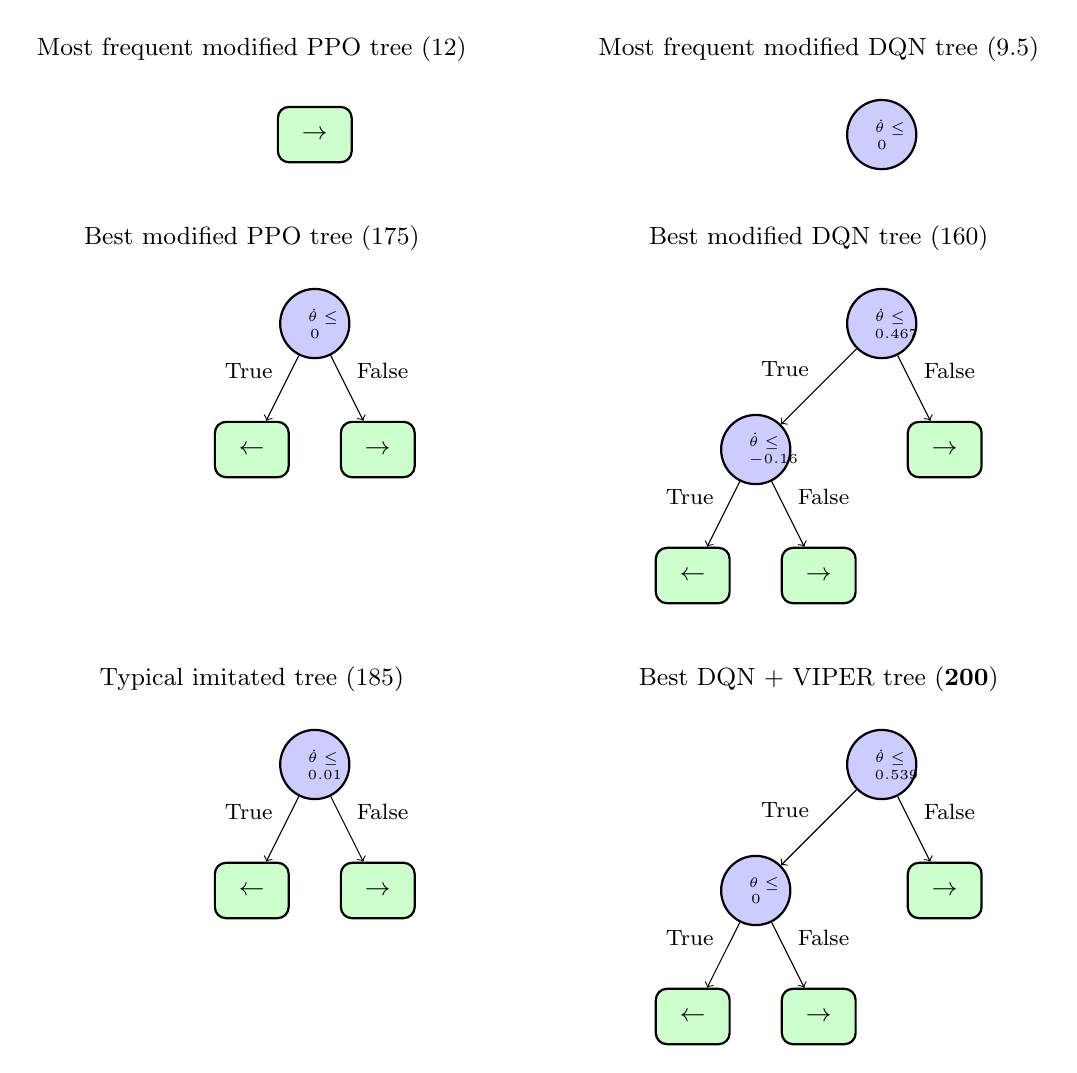
\begin{tikzpicture}[
        scale=0.8,
        decision/.style={circle, draw, thick, fill=blue!20, text width=0.5em, text centered, minimum height=2.5em, font=\tiny},
        leaf/.style={rectangle, draw, thick, fill=green!20, text width=2em, text centered, rounded corners, minimum height=2em, font=\small},
        edge_label/.style={font=\footnotesize, midway}
    ]

        \node[leaf] (tree7_root) at (-3,3) {$\rightarrow$};
        % \draw[->] (tree7_root) to[out=45,in=0,looseness=5] (tree7_root);

        \node[decision] (tree7_root) at (6,3) {$\dot{\theta} \leq 0$};
        % \draw[->] (tree7_root) to[out=45,in=0,looseness=5] (tree7_root);
        
        % Tree 4: if x <= 0.5 move right else move left
        \node[decision] (tree4_root) at (-3,0) { $\dot{\theta}\leq 0$};
        \node[leaf] (tree4_right) at (-4,-2) {$\leftarrow$};
        \node[leaf] (tree4_left) at (-2,-2) {$\rightarrow$};
        \draw[->] (tree4_root) -- (tree4_right) node[edge_label, above left] {True};
        \draw[->] (tree4_root) -- (tree4_left) node[edge_label, above right] {False};
        

        % Tree 7: if x <= 0.5 and y <= 0.5 move right else move down
        \node[decision] (tree7_root) at (6,0) {$\dot{\theta}\leq 0.467$};
        \node[decision] (tree7_y) at (4,-2) {$\dot{\theta}\leq -0.16$};
        \node[leaf] (tree7_right) at (3,-4) {$\leftarrow$};
        \node[leaf] (tree7_down) at (5,-4) {$\rightarrow$};
        \node[leaf] (tree7_down2) at (7,-2) {$\rightarrow$};
        \draw[->] (tree7_root) -- (tree7_y) node[edge_label, above left] {True};
        \draw[->] (tree7_root) -- (tree7_down2) node[edge_label, above right] {False};
        \draw[->] (tree7_y) -- (tree7_right) node[edge_label, above left] {True};
        \draw[->] (tree7_y) -- (tree7_down) node[edge_label, above right] {False};




        % Tree 4: if x <= 0.5 move right else move left (Second row, left)
        \node[decision] (tree4_root2) at (-3,-7) { $\dot{\theta}\leq 0.01$};
        \node[leaf] (tree4_right2) at (-4,-9) {$\leftarrow$};
        \node[leaf] (tree4_left2) at (-2,-9) {$\rightarrow$};
        \draw[->] (tree4_root2) -- (tree4_right2) node[edge_label, above left] {True};
        \draw[->] (tree4_root2) -- (tree4_left2) node[edge_label, above right] {False};


        % Tree 7: if x <= 0.5 and y <= 0.5 move right else move down (Second row, right)
        \node[decision] (tree7_root2) at (6,-7) {$\dot{\theta}\leq 0.539$};
        \node[decision] (tree7_y2) at (4,-9) {$\theta\leq 0$};
        \node[leaf] (tree7_right2) at (3,-11) {$\leftarrow$};
        \node[leaf] (tree7_down3) at (5,-11) {$\rightarrow$};
        \node[leaf] (tree7_down4) at (7,-9) {$\rightarrow$};
        \draw[->] (tree7_root2) -- (tree7_y2) node[edge_label, above left] {True};
        \draw[->] (tree7_root2) -- (tree7_down4) node[edge_label, above right] {False};
        \draw[->] (tree7_y2) -- (tree7_right2) node[edge_label, above left] {True};
        \draw[->] (tree7_y2) -- (tree7_down3) node[edge_label, above right] {False};
        

        % Labels
        \node[above] at (-4,4) {{\small Most frequent modified PPO tree (12)}};
        \node[above] at (5,4) {{\small Most frequent modified DQN tree (9.5)}};

        \node[above] at (-4,1) {{\small Best modified PPO tree (175)}};
        \node[above] at (5,1) {{\small Best modified DQN tree (160)}};
        \node[above] at (-4,-6) {{\small Typical imitated tree (185)}};
        \node[above] at (5,-6) {{\small Best DQN + VIPER tree (\textbf{200})}};


    \end{tikzpicture}
    \caption{Trees obtained by modified deep RL in IBMDPs against trees obtained with imitation (RL objective value). $\theta$ and $\dot{\theta}$ are respectively the angle and the angular velocity of the pole}
    \label{fig:trees-drl}
\end{figure*}


On figure~\ref{fig:ppo-trees}, we isolate the best performing algorithms instantiations that learn decision tree policies for the CartPole MDP.
We compare the best modified DQN and modified PPO to imitation learning baselines that use the surrogate imitation objective (cf. definition~\ref{def:il}) to find CartPole decision tree policies.
We find that despite having poor performances in \textit{average}, the modified deep reinforcement learning baselines can find very good decision tree policies as shown by the min-max shaded areas on the left of figure~\ref{fig:ppo-trees} and the corresponding estimated density of learned trees performances.
However this is not desirable, a user typically wants an algorithm that can consistently find good decision tree policies.
As shown by the estimated densities, indirect methods consistently find good decision tree policies (the higher modes of distributions are on the right of the plot).
On the other hand, the decision tree policies returned by direct RL methods seem equally distributed on both extremes of the scores.

On figure~\ref{fig:trees-drl}, we present the best decision tree policies for CartPole returned by modified DQN and modified PPO.
We used algorithm~\ref{alg:extract-tree} to extract 20 trees from the 20 partially observable policies returned by the modified deep reinforcement learning algorithms over the 20 training seeds.
We then plot the best tree for each baseline.
Those trees get an average RL objective of roughly 175.
Similarly, we plot a representative tree for imitation learning baseline as well as a tree that is optimal for CartPole w.r.t. the RL objective obtained with VIPER. 
Unlike for direct methods, the trees returned by imitation learning are extremely similar across seeds. In particular they often only vary in the scalar value used in the root node but in general have the same structure and test the angular velocity.
On the other hand the most frequent trees across seeds returned by modified RL baselines are ``trivial'' decision tree policies that either repeat the same base action forever or repeat the same IGA (cf. definition~\ref{def:ibmdp}) forever.

We have shown that compared to learning non-interpretable but standard Markovian neural network policies for the base MDP or some associated IBMDP, reinforcement learning of partially observable policies in IBMDP is less efficient (cf. figures~\ref{fig:res-dqn} and~\ref{fig:res-ppo}). 
As a consequence, only a handful of modified RL runs are able to learn decision tree policies that are on par with imitated trees (cf. figure~\ref{fig:ppo-trees}).
In the next chapter, we highlight the connections between direct interpretable RL (cf. definition~\ref{def:irl}) and POMDPs to get insights on the hardness of direct reinforcement learning of decision trees.

From the previous chapter, we know that to directly learn decision tree policies that optimize the RL objective (cf. definition~\ref{def:mdp-obj}) for an MDP (cf. definition~\ref{def:mdp}), one can learn a deterministic partially observable policy that optimizes the interpretable RL objective (cf. definition~\ref{def:irl}) in an IBMDP (cf. definition~\ref{def:ibmdp} and proposition~\ref{def:po-policy}).
Such problems are classical instances of partially observable Markov decision processes (POMDPs)~\cite{POMDP,chap2}.
This connection with POMDPs brings novel insights to direct reinforcement learning of decision tree policies. 
In this chapter, all the decision processes have a finite number of vector-valued states and observations.
Hence we will use bold fonts for states and observations but we can still use summations rather than integrals when required.

\section{Partially observable iterative Markov decision processes}\label{sec:poibmdp}
A POMDP is an MDP where the current state is hidden; only some information about the current state is observable.

\begin{definition}[Partially observable Markov decision process]\label{def:pomdp}
A partially observable Markov decision process is a tuple $\langle X, A, O, R, T, T_0, \Omega\rangle$ where:
\begin{itemize}
    \item $X$ is the hidden state space.
    \item $A$ is a finite set of actions.
    \item $O$ is a set of observations.
    \item $T: X \times A \rightarrow \Delta(X)$ is the transition function, where $T(\boldsymbol{x}_t, a, \boldsymbol{x}_{t+1}) = P(\boldsymbol{x}_t|\boldsymbol{x}_{t+1}, a)$ is the probability of transitioning to state $\boldsymbol{x}_{t}$ when taking action $a$ in state $\boldsymbol{x}$
    \item $T_0$: is the initial distribution over states. 
    \item $\Omega: X \rightarrow \Delta(O)$ is the observation function, where $\Omega(\boldsymbol{o}, a, \boldsymbol{x}) = P(\boldsymbol{o}|\boldsymbol{x}, a)$ is the probability of observing $\boldsymbol{o}$ in state $\boldsymbol{x}$
    \item $R: X \times A \rightarrow \mathbb{R}$ is the reward function, where $R(\boldsymbol{x}, a)$ is the immediate reward for taking action $a$ in state $\boldsymbol{x}$
\end{itemize}
Note that $\langle X, A, R, T, T_0 \rangle$ defines an MDP.
\end{definition}

Let us define explicitly a partially observable iterative bounding Markov decision process (POIBMDP). It is essentially an IBMDP for which we explicitly define an observation space and an observation function:
\begin{definition}[Partially observable iterative bounding Markov decision process]\label{def:poibmdp} a partially observable iterative bounding Markov decision process $\mathcal{M}_{POIB}$ is a tuple:
    \begin{align*}
        \langle \overbrace{S\times O}^{\text{States}}, \underbrace{A\cup A_{info}}_{Action space},\overbrace{O}_{\text{Observations}} ,\underbrace{(R, \zeta)}^{Rewards}, \overbrace{(T_{info}, T, T_0)}_{Transitions}, \Omega \rangle
    \end{align*}
    , where $\langle S\times O, A\cup A_{info}, (R, \zeta),( T, T_0, T_{info})\rangle$ is an IBMDP (cf. definition~\ref{def:ibmdp}).
    The transition function $\Omega$ maps concatenation of state features and observations--IBMDP states--to observations, $\Omega:S\times O \rightarrow O$, with $P(\boldsymbol{o}|(\boldsymbol{s}, \boldsymbol{o}))=1$ 
\end{definition}

One can see POIBMDPs as particular instances of POMDPs where the observation function simply applies a mask over some features of the hidden state.
This setting has other names in the literature.
For example, POIBMDPs are mixed observability MDPs \cite{momdp} with base MDP state features as the \textit{hidden variables} and feature bounds as \textit{visible} variables.
POIBMDPs can also be seen as non-stationary MDPs (N-MDPs)~\cite{learning-pomdp} in which there is one different transition function per base MDP state: these are called hidden-mode MDPs~\cite{hmmdp}.
Following~\cite{learning-pomdp} we can write the value of a deterministic partially observable policy $\pi:O\rightarrow A\cup A_{info}$ in observation $\boldsymbol{o}$.

\begin{definition}[Partially observable value function]\label{def:vpo} In a POIBMDP (cf. definition~\ref{def:poibmdp}), the expected cumulative discounted reward of a deterministic partially observable policy $\pi:O\rightarrow A\cup A_{info}$ starting from observation $o$ is $V^{\pi}(\boldsymbol{o})$:
    \begin{align*}
        V^{\pi}(\boldsymbol{o}) &= \underset{(s,\boldsymbol{o}')\in S\times O}{\sum}P^{\pi}((\boldsymbol{s}, \boldsymbol{o}')|\boldsymbol{o})V^{\pi}((\boldsymbol{s}, \boldsymbol{o}'))
    \end{align*}
with $P^{\pi}((\boldsymbol{s}, \boldsymbol{o}')|\boldsymbol{o})$ the asymptotic occupancy distribution (see \cite[section 4]{learning-pomdp} for the full definition) of the hidden POIBMDP state $(\boldsymbol{s},\boldsymbol{o}')$ given the partial observation $o$ and $V^{\pi}((s, o'))$ the classical state-value function (cf. definition~\ref{def:vs}).
We abuse notation and denote both values of observations and values of states by $V$ since the function input is not ambiguous.
\end{definition}

The asymptotic occupancy distribution is the probability of a policy $\pi$ to arrive in $(s,\boldsymbol{o}')$ while observing $\boldsymbol{o}$ in some trajectory.  
In this chapter, we use reinforcement learning to train decision tree policies for MDPs by seeking deterministic partially observable policies that optimize the interpretable RL objective (cf. definition~\ref{def:irl}) in POIBMDPs (cf. definition~\ref{def:poibmdp}).
% We summarized the approach in figure~\ref{fig:summary-rl}  

% \begin{figure}
% \centering
% \begin{tikzpicture}
%     \draw[fill=blue!40] (0, 0) rectangle (6, 4);
%     \node at (3, 3.5) {POIBMDP $\mathcal{M}_{POIB}\langle\mathcal{M}_{IB}, O, \Omega\rangle$};
%     \draw[fill=blue!30] (0, 0) rectangle (5.9, 3);
%     \node at (3, 2.5) {IBMDP $\mathcal{M}_{IB} \langle \mathcal{M}, A_{info}, \zeta \rangle$};
%     \draw[fill=blue!10] (0, 0) rectangle (5, 2);
%     \node at (3, 1.5) {MDP $\mathcal{M} \langle S, A, R, T, T_0 \rangle$};
    
%     \draw[fill=red!10] (10, 0) rectangle (14, 3);
%     \node at (12, 2) {\textbf{Objective~\ref{def:irl}}};
%     \node at (12, 1) {$\pi^{\star} = \underset{\pi}{\operatorname{argmax}} V^{\pi}(\boldsymbol{o}_0)$};
    
%     \draw[fill=red!10] (1, -5) rectangle (5, -2);
%     \node at (3, -3) {\textbf{Decision Tree Policy}};
%     \node at (3, -4) {$\pi_{\mathcal{T}}: S \rightarrow A$};
    
%     \draw[fill=red!10] (9.5, -5) rectangle (14.5, -2);
%     \node at (12, -3) {\textbf{Deterministic policy}};
%     \node at (12, -4) {$\pi: O \rightarrow A \cup A_{info}$};
    
%     \draw[thick, ->] (6, 2) -- (10, 2) node[midway, above] {$\gamma$};
%     \draw[thick, <-] (5, -3.5) -- (9.5, -3.5) node[midway, above] {Extract tree with algorithm\ref{alg:extract-tree}};
%     \draw[thick, ->] (12, 0) -- (12, -2) node[midway, left] {Solve with e.g. RL~\ref{sec:rl}};
%     \draw[thick, <-] (3, 0.5) -- (3, -2) node[midway, left] {Can be interpreted};

    
%     % % Final arrow from tree back to base MDP - adjusted position
%     % \draw[thick, ->] (1.75, -2.5) -- (1.75, -0.5) node[midway, right] {Can deploy\\and interpret};
    
% \end{tikzpicture}
% \caption{A formal framework to learn decision tree policies for MDPs that directly optimize a trade-off between the RL objective~\ref{def:mdp-obj} and interpretability.
% This framework relies on learning a deterministic partially observable policy in a POIBMDP~\ref{def:poibmdp}.}
% \label{fig:summary-rl}
% \end{figure}
The goal of the following sections is to see if, unlike indirect approaches tested in section~\ref{sec:limits-il} (cf. figures~\ref{fig:objectives} and~\ref{fig:ql-il}), direct approaches can consistently learn the depth-1 decision tree policies that have good interpretability-performance trade-offs for the $2\times 2$ grid world from example~\ref{example:grid} (cf. figures~\ref{fig:trees-intro} and~\ref{fig:optimal-policy-trees}).
The direct approach optimizes the interpretable RL objective~\ref{def:irl} in POIBMDPs (cf. definition~\ref{def:poibmdp}).
We will use reinforcement learning to learn deterministic partially observable policies for the IBMDP from example~\ref{example:ibmdp} re-written as a POIBMDP.
Next we show how to choose $\gamma$ and $\zeta$ in the POIBMDP such that the optimal deterministic partially observable policies w.r.t. the interpretable RL objective correspond exactly to the depth-1 decision tree policies with good interpretability-performance trade-offs.
Hence, if we find that RL can consistently find optimal policies w.r.t. interpretable RL objective, it means that this direct approach can consistently find the depth-1 decision tree policies with good interpretability-performance trade-off that indirect approaches could not consistently find.

\section{Constructing POIBMDPs whose optimal solutions are depth-1 decision tree policies}\label{sec:opt-depth1}
\begin{figure}
    \centering
    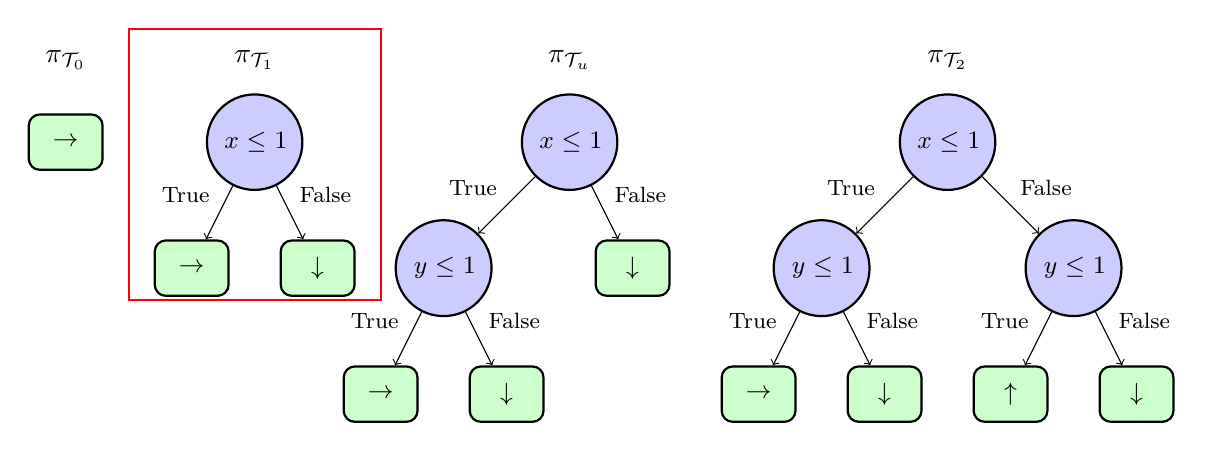
\begin{tikzpicture}[
        scale=0.8,
        decision/.style={circle, draw, thick, fill=blue!20, text width=2.5em, text centered, minimum height=2.5em, font=\small},
        leaf/.style={rectangle, draw, thick, fill=green!20, text width=2em, text centered, rounded corners, minimum height=2em, font=\small},
        edge_label/.style={font=\footnotesize, midway}
    ]
        
        \node[leaf] at (-3, 0) {$\rightarrow$};
        % Tree 4: if x <= 0.5 move right else move left
        \node[decision] (tree4_root) at (0,0) {$x \leq 1$};
        \node[leaf] (tree4_right) at (-1,-2) {$\rightarrow$};
        \node[leaf] (tree4_left) at (1,-2) {$\downarrow$};
        \draw[->] (tree4_root) -- (tree4_right) node[edge_label, above left] {True};
        \draw[->] (tree4_root) -- (tree4_left) node[edge_label, above right] {False};
        
        % Draw a square around the tree
        \draw[thick, red] (-2, 1.8) rectangle (2, -2.5);

        % Tree 7: if x <= 0.5 and y <= 0.5 move right else move down
        \node[decision] (tree7_root) at (5,0) {$x \leq 1$};
        \node[decision] (tree7_y) at (3,-2) {$y \leq 1$};
        \node[leaf] (tree7_right) at (2,-4) {$\rightarrow$};
        \node[leaf] (tree7_down) at (4,-4) {$\downarrow$};
        \node[leaf] (tree7_down2) at (6,-2) {$\downarrow$};
        \draw[->] (tree7_root) -- (tree7_y) node[edge_label, above left] {True};
        \draw[->] (tree7_root) -- (tree7_down2) node[edge_label, above right] {False};
        \draw[->] (tree7_y) -- (tree7_right) node[edge_label, above left] {True};
        \draw[->] (tree7_y) -- (tree7_down) node[edge_label, above right] {False};


        \node[decision] (tree7_root) at (11,0) {$x \leq 1$};
        \node[decision] (tree7_y) at (9,-2) {$y \leq 1$};
        \node[decision] (tree7_y2) at (13,-2) {$y \leq 1$};
        \node[leaf] (tree7_right) at (8,-4) {$\rightarrow$};
        \node[leaf] (tree7_down) at (10,-4) {$\downarrow$};
        \node[leaf] (tree7_right2) at (12,-4) {$\uparrow$};
        \node[leaf] (tree7_down2) at (14,-4) {$\downarrow$};
        \draw[->] (tree7_root) -- (tree7_y) node[edge_label, above left] {True};
        \draw[->] (tree7_root) -- (tree7_y2) node[edge_label, above right] {False};
        \draw[->] (tree7_y) -- (tree7_right) node[edge_label, above left] {True};
        \draw[->] (tree7_y) -- (tree7_down) node[edge_label, above right] {False};
        \draw[->] (tree7_y2) -- (tree7_right2) node[edge_label, above left] {True};
        \draw[->] (tree7_y2) -- (tree7_down2) node[edge_label, above right] {False};

        % Labels
        \node[above] at (-3,1) {$\pi_{\mathcal{T}_0}$};
        \node[above] at (0,1) {$\pi_{\mathcal{T}_1}$};
        \node[above] at (5,1) {$\pi_{\mathcal{T}_u}$};
        \node[above] at (11,1) {$\pi_{\mathcal{T}_2}$};


    \end{tikzpicture}
    \caption{For each decision tree structure, e.g., depth-1 or unbalanced depth-2, we illustrate a decision tree which maximizes the RL objective (cf. definition~\ref{def:mdp-obj}) in the grid world MDP.}
    \label{fig:optimal-policy-trees}
\end{figure}

Because we know all the base states, all the observations, all the actions, all the rewards and all the transitions of our POIBMDP (cf. example~\ref{example:ibmdp}), we can compute exactly the values of different deterministic partially observable policies given, $\zeta$ the reward for IGAs, and $\gamma$ the discount factor.
Each of those policies can be one of the trees illustrated in figure~\ref{fig:optimal-policy-trees}: 

\begin{itemize}
    \item $\pi_{\mathcal{T}_0}$: a depth-0 tree equivalent to always taking the same base action 
    \item $\pi_{\mathcal{T}_1}$: a depth-1 tree equivalent alternating between an IGA and a base action 
    \item $\pi_{\mathcal{T}_u}$: an unbalanced depth-2 tree that sometimes takes two IGAs then a base action and sometimes a an IGA then a base action
    \item $\pi_{\mathcal{T}_2}$: a depth-2 tree that alternates between taking two IGAs and a base action
    \item an infinite ``tree'' that only takes IGAs
\end{itemize}
Furthermore, because from~\cite{learning-pomdp} we know that for POMDPs, stochastic partially observable policies can sometimes get better expected discounted rewards than deterministic partially observable policies, we also compute the value of the stochastic policy that randomly alternates between two base actions: $\rightarrow$ and $\downarrow$.
Those two base actions always lead to the goal state (cf. figure~\ref{example:grid}).

\begin{proposition}[Depth-1 decision tree objective value] The interpretable RL objective value (cf. definition~\ref{def:irl}) of depth-1 decision tree policies with good interpretability–performance trade-offs in the grid world MDP (cf. figures~\ref{fig:trees-intro} and~\ref{fig:optimal-policy-trees}) is $\frac{4\zeta + \gamma + 2\gamma^3 + \gamma^5}{4(1-\gamma^2)}$.
\end{proposition}

We defer the lengthy proofs of this proposition, as well as the interpretable RL objective values of other decision tree policies, to the appendix~\ref{calcs}.

\begin{figure}
    \centering
    \includegraphics[width=0.6\textwidth]{../images/images_part1/objective_values_plot.pdf}
    \caption{Interpretable RL objective values (cf. definition~\ref{def:irl}) of different partially observable policies as functions of $\zeta$. Shaded areas show the optimal \textit{deterministic} partially observable policies in different ranges of $\zeta$ values.}\label{fig:irl-objectives}
\end{figure}

We can now plot, in figure~\ref{fig:irl-objectives}, the interpretable RL objective values of the different partially observable policies as functions of $\zeta$ when we fix $\gamma=0.99$. 
When $\gamma=0.99$, despite objective values being very similar for the depth-1 and unbalanced depth-2 tree, we now know from the green shaded area that a depth-1 tree is the optimal one, w.r.t. the interpretable RL objective, deterministic partially observable POIBMDP policy for $0< \zeta < 1$.

Let us now define a POIBMDP with the grid world (cf. figure~\ref{example:grid}) as the base MDP, with IGAs as in the IBMDP from example~\ref{example:ibmdp}, with $\gamma=0.99$ and $0<\zeta<1$ and verify if RL can learn the optimal deterministic partially observable policies w.r.t. the interpretable RL objective, which are equivalent to depth-1 decision tree policies, in this very controlled experiment.

\section{Reinforcement learning in PO(IB)MDPs}

In general, the policy that maximizes the RL objective (cf. definition~\ref{def:mdp-obj}) in a POMDP (cf. definition~\ref{def:pomdp}) maps ``belief states'' or observation histories~\cite{chap2} to actions. Hence, those policies are not solutions to our problem since we require that policies depend only on the current observation.
If we did not have this constraint, we could apply any standard RL algorithm to solve POIBMDPs by seeking such policies because both histories and belief states are sufficient statistics for POMDP hidden states~\cite{chap2,lambrechts2025informed}.

In particular, the problem of finding the optimal deterministic partially observable policies for POMDPs is NP-HARD, even with full knowledge of transitions and rewards~\cite[section 3.2]{littman1}.
It means that it is impractical to enumerate all possible policies and take the best one. 
For even moderate-sized POMDPs, a brute-force approach would take a very long time since there are $|A|^{|O|}$ deterministic partially observable policies.
Hence it is interesting to study reinforcement learning for finding the best deterministic partially observable policy since it would not search the whole solution space.
However applying RL to our interpretable RL objective (cf. definition~\ref{def:irl}) is non-trivial.

In~\cite[Fact 2]{learning-pomdp}, the authors show that the optimal partially observable policy can be stochastic. Hence, policy gradient algorithms~\cite{pg_sutton}--that return stochastic policies--are to avoid since we seek the best \textit{deterministic} policy. 
Furthermore, the optimal deterministic partially observable policy might not maximize all the values of all observations simultaneously ~\cite[Fact 5]{learning-pomdp} which makes it difficult to use TD-learning (cf. algorithms~\ref{alg:qlearning} and~\ref{alg:sarsa}).
Indeed, doing a TD-learning update of one partially observable value (cf. definition~\ref{def:vpo}) with, e.g. Q-learning, can change the value of \textit{all} other observations in an uncontrollable manner because of the dependence in $P^{\pi}((s, \boldsymbol{o}')|\boldsymbol{o})$ (cf. definition~\ref{def:vpo}).
Interestingly, those two challenges of learning in POMDPs described in \cite{learning-pomdp} are visible in figure~\ref{fig:irl-objectives}. 
First, there is a whole range of $\zeta$ values for which the optimal partially observable policy is stochastic.
Second, for e.g. $\zeta=0.5$, while a depth-1 tree is the optimal deterministic partially observable policy, the value of state $(\boldsymbol{s}_2, \boldsymbol{o}_0) = (1.5, 1.5, 0, 2, 0, 2)$ is not maximized by this partially observable policy but by the sub-optimal policy that always goes down.

Despite those hardness results, empirical results of applying RL to POMDPs by naively replacing $\boldsymbol{x}$ by $\boldsymbol{o}$ in Q-learning or Sarsa, has already demonstrated successful in practice~\cite{sarsa-pomdp}. 
More recently, the framework of Baisero et. al. called asymmetric RL~\cite{baisero-dqn,baisero-ppo} has also shown promising results to learn POMDP solutions.
Asymmetric RL algorithms train a model--a policy or a value function--depending on hidden state (only available at train time) and a history dependent (or observation dependent) model.
The history or observation dependent model serves as target or critic to train the hidden state dependent model.
The history dependent (or observation dependent) model can thus be deployed in the POMDP after training since it does not require access to the hidden state to output actions.
In algorithm~\ref{alg:asymqlearning} we present asymmetric Q-learning. It is a variant of Q-learning (cf. algorithm~\ref{alg:qlearning}) that returns a deterministic partially observable policy like modified DQN~\ref{alg:mod-dqn}.
Given a POMDP, asymmetric Q-learning trains a partially observable Q-function $Q:O\times A\rightarrow\mathbb{R}$ and a Q-function $U:X\times A\rightarrow\mathbb{R}$. The hidden state dependent Q-function $U$ serves as a target in the temporal difference learning update. 
We also consider an asymmetric version of Sarsa that applies similar modifications to the standard Sarsa (cf. algorithm~\ref{alg:sarsa}). We present asymmetric Sarsa in the appendix (cf. algorithm~\ref{alg:asymsarsa}).
In~\cite{jsj}, the authors introduce a policy search algorithm~\ref{sec:rl} that learns a (stochastic) policy $\pi:O\rightarrow\Delta(A)$ and a critic $V:X\rightarrow \mathbb{R}$ using Monte Carlo estimates to guide policy improvement.
We also consider this algorithm in our experiments that we call JSJ (for the authors names Jaakkola, Singh, Jordan). We present the JSJ algorithm in the appendix (cf. algorithm~\ref{alg:jsj}).
JSJ is equivalent to a tabular asymmetric policy gradient algorithm (cf. algorithm~\ref{alg:reinforce}). 

Until recently, the benefits of asymmetric RL over standard RL was only shown empirically and only for history-dependent models.
The work of Gaspard Lambrechts~\cite{justif-asym} proves that some asymmetric RL algorithms learn better history-dependent \textbf{or} partially observable policies for solving POMDPs.
This is exactly what we wish for. However, those algorithms are not practical because they require estimations of the asymptotic occupancy distribution $P^{\pi}((s, \boldsymbol{o}')|\boldsymbol{o})$ (cf. definition~\ref{def:vpo}) for candidate policies which in turn would require to gather a lot of on-policy samples.
We leave it to future work to use those algorithms that combine asymmetric RL and estimation of future visitation frequencies since those results are contemporary to the writing of this manuscript.

Note that, in the previous chapter and in the original work of Topin et. al.~\cite{topin2021iterative}, modified DQN (cf. algorithm~\ref{alg:mod-dqn}) and modified PPO (cf. algorithm~\ref{alg:mod-ppo}) are respectively asymmetric DQN and asymmetric PPO from~\cite{baisero-dqn,baisero-ppo}.
In the next section, we use (asymmetric) RL to optimize the interpretable RL objective in POIBMDPs.
\RestyleAlgo{ruled}
\SetKwComment{Comment}{}{}
\begin{algorithm}
    \KwData{POMDP $\mathcal{M}_{po} = \langle X, O, A, R, T, T_0, \Omega \rangle$, learning rates $\alpha_u,\quad \alpha_q$, exploration rate $\epsilon$}
    \KwResult{$\pi:O\rightarrow A$}
    \textcolor{green}{Initialize $U(\boldsymbol{x},a) = 0$ for all $x \in X, a \in A$ \\}
    Initialize $Q(\boldsymbol{o},a) = 0$ for all $o \in O, a \in A$ \\

    \For{each episode}{
        Initialize state $x_0 \sim T_0$ \\
        Initialize observation $\boldsymbol{o}_0 \sim \Omega(\boldsymbol{x}_0)$ \\

        \For{each step $t$}{
            Choose action $a_t$ using $\epsilon$-greedy: $a_t = \operatorname{argmax}_a Q(\boldsymbol{o}_t,a)$ with prob. $1-\epsilon$ \\
            Take action $a_t$, observe $r_t = R(\boldsymbol{x}_t,a_t)$, $x_{t+1} \sim T(x_t,a_t)$, and $\boldsymbol{o}_{t+1} \sim \Omega(\boldsymbol{x}_{t+1})$ \\
            \textcolor{green}{$y \leftarrow r + \gamma U(\boldsymbol{x}_{t+1}, \operatorname{argmax}_{a'} Q(\boldsymbol{o}_{t+1}, a'))$} \Comment{// TD target} \\
            $U(\boldsymbol{x}_t,a_t) \leftarrow (1 - \alpha_u) U(\boldsymbol{x}_t, a_t) + \alpha_u y $ \\
            \textcolor{green}{$Q(\boldsymbol{o}_t,a_t) \leftarrow (1 - \alpha_q) Q(\boldsymbol{o}_t, a_t) + \alpha_q y $} \\
            $x_t \leftarrow \boldsymbol{x}_{t+1}$ \\
            $\boldsymbol{o}_t \leftarrow \boldsymbol{o}_{t+1}$ \\
        }
    }
    $\pi(o) = \operatorname{argmax}_a Q(\boldsymbol{o},a)$ \Comment{// Extract greedy policy}
    \caption{Asymmetric Q-Learning. We highlight in green the differences with the standard Q-learning (cf. algorithm~\ref{alg:qlearning})}\label{alg:asymqlearning}
\end{algorithm}

In the next section, we apply asymmetric and standard RL algorithms to the problem of learning the optimal depth-1 tree for the grid world MDP (cf. section~\ref{sec:opt-depth1}) by optimizing the interpretable RL objective in POIBMDPs.

\section{Results}

The results presented in the section show that (asymmetric) reinforcement learning fails for the aforementioned problem. Let us understand why.

\subsection{Experimental setup}

\paragraph{Baselines:} we consider two groups of RL algorithms.
The first group is standard tabular RL algorithms to optimize the interpretable RL objective in POIBMDPs; Q-learning, Sarsa, and Policy Gradient with a softmax policy (cf. section~\ref{sec:rl}, algorithms~\ref{alg:qlearning},~\ref{alg:sarsa}, and~\ref{alg:reinforce}).
In theory the Policy Gradient algorithm should not be a good candidate for our problem since it searches for stochastic policies that we showed can be better than our sought depth-1 decision tree policy (cf. figure~\ref{fig:irl-objectives}).

In addition to the traditional tabular RL algorithms above, we also apply asymmetric Q-learning, asymmetric Sarsa, and JSJ (algorithms~\ref{alg:asymqlearning},~\ref{alg:asymsarsa} and~\ref{alg:jsj}).
We use at least 200 000 POIBMDP time steps per experiment. Each experiment, i.e an RL algorithm learning in a POIBMDP, is repeated 100 times.  

\paragraph{Hyperparameters:} For all baselines we use, when applicable, exploration rates $\epsilon=0.3$ and learning rates $\alpha=0.1$.

\paragraph{Metrics:} We will consider two metrics.
First, the sub-optimality gap during training, w.r.t. the interpretable RL objective, between the learned partially observable policy and the optimal deterministic partially observable policy: $|\mathbb{E}\left[V^\pi^{\star}(\boldsymbol{s}_0,\boldsymbol{o}_0)| \boldsymbol{s}_0\sim T_0\right] - \mathbb{E}\left[V^\pi(\boldsymbol{s}_0,\boldsymbol{o}_0)|\boldsymbol{s}_0\sim T_0\right]|$.
Because we know the whole POIBMDP model that we can represent exactly as tables, and because we know for each $\zeta$ the interpretable RL objective value of the optimal deterministic partially observable policy (cf. figure~\ref{fig:irl-objectives}), we can report the \textit{exact} sub-optimality gaps.

Second, we consider the distribution of the learned trees over the 100 training seeds.
Indeed, since for every POIBMDP we run each algorithm 100 times, at the end of training we get 100 deterministic partially observable policies (we compute the greedy policy for stochastic policies returned by JSJ and Policy Gradient), from which we can extract the equivalent 100 decision tree policies using algorithm~\ref{alg:extract-tree} and we can count which one are of e.g. depth 1.
This helps understand which trees RL algorithms tend to learn.

\subsection{Can (asymmetric) RL learn optimal deterministic partially observable POIBMDP policies?}

In figure~\ref{fig:rl-poibmdp}, we plot the sub-optimality gaps--averaged over 100 seeds--of learned policies during training.
We do so for 200 different POIBMDPs where we change the reward for information gathering actions: we sample 200 $\zeta$ values uniformly in $[-1, 2]$.
In figure~\ref{fig:rl-poibmdp}, a different color represents a different POIBMDP.

Recall from figure~\ref{fig:irl-objectives} that for:
\begin{itemize}
    \item $\zeta\in [-1, 0]$, the optimal deterministic partially observable policy is a depth-0 tree
    \item $\zeta\in ]0, 1[$, the optimal deterministic partially observable policy is a depth-1 tree
    \item $\zeta\in [1, 2]$, the optimal deterministic partially observable policy is a ``infinite'' tree that contains infinite number of internal nodes.
\end{itemize}
We observe that, despite all sub-optimality gaps converging independently of the $\zeta$ values, not all algorithms in all POIBMDPs fully minimize the sub-optimality gap.
In particular, all algorithms seem to consistently minimize the gap, i.e. learn the optimal policy or Q-function, only for $\zeta \in [1, 2]$ (all the yellow lines go to 0).
However, we are interested in the range $\zeta\in ]0, 1[$ where the optimal decision tree policy is non-trivial, i.e. not taking the same action forever.
In that range, no baseline consistently minimizes the sub-optimality gap.


In figure~\ref{fig:dt-distrib-poibmdp}, we plot the distributions of the final learned trees over the 100 random seeds in function of $\zeta$ from the above runs.
For example, in figure~\ref{fig:dt-distrib-poibmdp}, in the top left plot, when learning 100 times in a POIBMDP with $\zeta=0.5$, Q-learning returned almost 100 times a depth-0 tree.
Again, on none of those subplots do we see a high rate of learned depth-1 trees for $\zeta\in ]0, 1[$.
It is alerting that the most frequent learned trees are the depth-0 trees for $\zeta\in ]0, 1[$ because such trees are way more sub-optimal w.r.t. the interpretable RL objective (cf. definition~\ref{def:irl}) than e.g. the depth-2 unbalanced trees (cf. figure~\ref{fig:irl-objectives}).  
One interpretation of this phenomenon is that the learning in POIBMDPs is very difficult and so agents tend to converge to trivial policies, e.g., repeating the same base action.

However, on the positive side, we observe that asymmetric versions of Q-learning and Sarsa have found the optimal deterministic partially observable policy--the depth-1 decision tree--more frequently throughout the optimality range $]0,1[$, than their symmetric counter-parts for $\zeta\in ]0, 1[$.
Next, we quantify how difficult it is to do RL to learn partially observable policies in POIBMDPs.

\begin{figure}
    \centering
    \includegraphics[width=1\textwidth]{../images/images_part1/learning_curves.pdf}
    \caption{(Asymmetric) reinforcement learning in POIBMDPs. 
    In each subplot, each single line is colored by the value of $\zeta$ in the corresponding POIBMDP in which learning occurs. 
    Each single learning curve represent the sub-optimality gap averaged over 100 seeds.
    }\label{fig:rl-poibmdp}
\end{figure}

\begin{figure}
    \centering
    \includegraphics[width=1\textwidth]{../images/images_part1/tree_distributions.pdf}
    \caption{Distributions of final tree policies learned across the 100 seeds.
    For each $\zeta$ value, there are four colored points. Each point represent the share of depth-0 trees (red), depth-1 trees (green), unbalanced depth-2 trees (orange) and depth-2 trees (blue).
    }\label{fig:dt-distrib-poibmdp}
\end{figure}


\subsection{How difficult is it to learn in POIBMDPs?}\label{sec:how-diff}

In this section we run the same (asymmetric) reinforcement learning algorithms to optimize either the RL objective (cf. definition~\ref{def:mdp-obj}) in MDPs (cf. definition~\ref{def:mdp}) or IBMDPs (cf. definition~\ref{def:ibmdp}), or the interpretable RL objective in POIBMDPs(cf. definition~\ref{def:irl}).
This essentially results in three distinct problems:
\begin{enumerate}
    \item Learning an optimal standard Markovian policy in an MDP, i.e. optimizing the RL objective in an MDP.
    \item Learning an optimal standard Markovian policy in an IBMDP, i.e. optimizing the RL objective in an IBMDP.
    \item Learning an optimal deterministic partially observable policy in a POIBMDP.
\end{enumerate}

In order to see how difficult each of these three problems is, we can run a \textit{great} number of experiments for each problem and compare solving rates.
To make solving rates comparable we consider a unique instance for each of those problems.
Problem 1 is learning one of the optimal standard Markovian deterministic policy from figure~\ref{example:grid} for the grid world from example~\ref{example:grid} with $\gamma=0.99$.
Problem 2 is learning one of the optimal standard Markovian deterministic for the IBMDP from figure~\ref{example:ibmdp} with $\gamma=0.99$ and $\zeta=0.5$.
This is similar to the previous chapter experiments where we applied DQN or PPO to an IBMDP for CartPole without constraining the search to partially observable policies (see e.g. figure\ref{fig:res-ppo}).
Problem 3 is what has been done in the previous section to learn deterministic partially observable policies where in addition of fixing $\gamma=0.99$ we also fix $\zeta=0.5$.

We use the six (asymmetric) RL algorithms from the previous section and try a wide set of hyperparameters and additional learning tricks (optimistic Q-function, eligibility traces, entropy regularization and $\epsilon$-decay, all are described in \cite{sutton}).
We only provide the detailed hyperparameters for asymmetric Sarsa and an overall summary for all the algorithms in tables~\ref{tab:hp-sarsa} and~\ref{tab:ib-params}.
The complete detailed lists of hyperparameters are given in the appendix~\ref{sec:hp-pomdp}.
Furthermore, the careful reader might notice that there is no point running asymmetric RL on MDPs or IBMDPs when the problem does not require partial observability.
Hence, we only run asymmetric RL for POIBMDPs and otherwise run all other RL algorithms and all problems.

Each unique hyperparameter combination for a given algorithm on a given problem is run 10 times on 1 million learning steps.
For example, for asymmetric Sarsa, we run a total of $10\times 768= 7680$ experiments for learning deterministic partially observable policies for a POIBMDP (cf. table~\ref{tab:hp-sarsa}).
To get a success rate, we can simply divide the number of learned depth 1 tree by 7680 (recall that for $\gamma=0.99$ and $\zeta=0.5$, the optimal policy is a depth-1 tree (e.g. figure~\ref{fig:optimal-policy-trees}) as per figure~\ref{fig:irl-objectives}). 

\begin{table}
\centering
\small
\caption{Asymmetric sarsa hyperparameters (768 combinations each run 10 times)}\label{tab:hp-sarsa}
\begin{tabular}{lll}
\toprule
\textbf{Hyperparameter} & \textbf{Values} & \textbf{Description} \\
\midrule
Epsilon Schedules & (0.3, 1), (0.3, 0.99), (1, 1) & Initial exploration and decrease rate \\
Epsilon Schedules & (0.1, 1), (0.1, 0.99), (0.3, 0.99) & Initial exploration and decrease rate \\
Lambda & 0.0, 0.3, 0.6, 0.9 & Eligibility trace decay \\
Learning Rate $U$ & 0.001, 0.005, 0.01, 0.1 & learning rate for \\
 & & the Q-function \\
Learning Rate $Q$ & 0.001, 0.005, 0.01, 0.1 & learning rate for the \\
 & & partial observation dependent Q-function \\
Optimistic & True, False & Optimistic initialization \\
\bottomrule
\end{tabular}
\end{table}

\begin{table}
    \centering
    \caption{Summary of RL baselines Hyperparameters}\label{tab:ib-params}
    \begin{tabular}{llr}
    \toprule
    \textbf{algorithm} & \textbf{Problem} & \textbf{Total Hyperparameter Combinations} \\
    \midrule
    Policy Gradient & PO/IB/MDP & 420 \\
    JSJ & POIBMDP & 15 \\
    Q-learning & PO/IB/MDP & 192 \\
    Asym Q-learning & POIBMDP & 768 \\
    Sarsa & PO/IB/MDP & 192 \\
    Asym Sarsa & POIBMDP & 768 \\
    \bottomrule
    \end{tabular}
    \end{table}


The key observations from figure~\ref{fig:po-vs-ib} is that reinforcement learning a deterministic partially observable policy in a POIBMDP, is way harder than learning a standard Markovian policy.
For example, Q-learning only finds the optimal solution (cf. definition~\ref{def:irl}) in only 3\% of the experiments while the same algorithms to optimize the standard RL objective (cf. definition~\ref{def:mdp-obj}) in an MDP or IBMDP found the optimal solutions 50\% of the time.
Even though asymmetry seems to increase performances; learning a decision tree policy for a simple grid world directly with RL using the framework of POIBMDP originally developed in~\cite{topin2021iterative} seems way too difficult and costly as successes might require a million steps for such a seemingly simple problem.
An other difficulty in practice that we did not cover here, is the choice of information gathering actions.
For the grid world MDP, choosing good IGAs ($x\leq1$ and $y\leq1$) is simple but what about more complicated MDPs: how to instantiate the (PO)IBMDP action space such that internal nodes in resulting trees are useful for predictions?

To go even further, on figure~\ref{fig:asym-ql-analysis} we re-run experiments from figure~\ref{fig:rl-poibmdp} and figure~\ref{fig:dt-distrib-poibmdp} using the top performing hyperparameters for asymmetric Q-learning (given in appendix~\ref{tab:algorithm-hyperparameters}).
While those hyperparameters resulted in asymmetric Q-learning returning 10 of out 10 times an optimal depth 1 tree,
the performances didn't transfer.
On figure~\ref{fig:asym-ql-analysis} despite higher success rates in the region $\zeta\in]0,1[$ compared to figure~\ref{fig:dt-distrib-poibmdp}. 

\begin{figure}
    \centering
    \includegraphics[width=0.8\textwidth]{../images/images_part1/algorithm_performance_comparison_flattened.pdf}
    \caption{Success rates of different (asymmetric) RL algorithms over thousands of runs when applied to learning deterministic partially observable policies in a POIBMDP or learning deterministic policies in associated MDP and IBMDP.}\label{fig:po-vs-ib}
\end{figure}


\begin{figure}
    \begin{subfigure}[b]{0.49\textwidth}
        \includegraphics[width=\textwidth]{../images/images_part1/ql_asym_best_learning_curves.pdf}
        \caption{Learning curves for asymmetric Q-learning with good hyperparameters.}
        \label{fig:best-learning-curves}
    \end{subfigure}
    \hfill
    \begin{subfigure}[b]{0.49\textwidth}
        \includegraphics[width=\textwidth]{../images/images_part1/ql_asym_best_tree_distributions.pdf}
        \caption{Trees distributions for asymmetric Q-learning with good hyperparameters}
        \label{fig:best-tree-distributions}
    \end{subfigure}
    \caption{Analysis of the top-performing asymmetric Q-learning instantiation. (left) Learning curves, and (right) tree distributions across different POIBMDP configurations.}
    \label{fig:asym-ql-analysis}
\end{figure}


\section{Conclusion}
In this chapter, we have shown that direct learning of decision tree policies for MDPs can be reduced to learning deterministic partially observable policies in POMDPs that we called POIBMDPs.
By crafting a POIBMDP for which we know exactly the optimal deterministic partially observable policy w.r.t. the interpretable RL objective (cf. definition~\ref{def:irl}), we were able to benchmark the sub-optimality of solutions learned with (asymmetric) reinforcement learning.

Across our experiments, we found that no algorithm could consistently learn a depth-1 decision tree policy for a grid world MDP despite it being optimal both w.r.t. the interpretable RL objective and standard RL objective (cf. definition~\ref{def:mdp-obj}).
When compared to the results of VIPER from figure~\ref{fig:ql-il}, direct RL is worse at retrieving decision tree policies with good interpretability-performance trade-offs.
This echoes the results from the previous chapter in which we saw that direct deep RL performed worse than imitation learning to find decision tree policies for CartPole.

In the next chapter, we find that RL can find optimal deterministic partially observable policies for a special class of POIBMDPs that we believe makes for a convincing argument as to why direct learning of decision tree policies that optimize the RL objective (cf. definition~\ref{def:mdp-obj}) is so difficult.


\bibliography{example_paper}
\bibliographystyle{icml2026}

%%%%%%%%%%%%%%%%%%%%%%%%%%%%%%%%%%%%%%%%%%%%%%%%%%%%%%%%%%%%%%%%%%%%%%%%%%%%%%%
%%%%%%%%%%%%%%%%%%%%%%%%%%%%%%%%%%%%%%%%%%%%%%%%%%%%%%%%%%%%%%%%%%%%%%%%%%%%%%%
% APPENDIX
%%%%%%%%%%%%%%%%%%%%%%%%%%%%%%%%%%%%%%%%%%%%%%%%%%%%%%%%%%%%%%%%%%%%%%%%%%%%%%%
%%%%%%%%%%%%%%%%%%%%%%%%%%%%%%%%%%%%%%%%%%%%%%%%%%%%%%%%%%%%%%%%%%%%%%%%%%%%%%%
\newpage
\appendix
\onecolumn
\section{You \emph{can} have an appendix here.}

You can have as much text here as you want. The main body must be at most $8$
pages long. For the final version, one more page can be added. If you want, you
can use an appendix like this one.

The $\mathtt{\backslash onecolumn}$ command above can be kept in place if you
prefer a one-column appendix, or can be removed if you prefer a two-column
appendix.  Apart from this possible change, the style (font size, spacing,
margins, page numbering, etc.) should be kept the same as the main body.
%%%%%%%%%%%%%%%%%%%%%%%%%%%%%%%%%%%%%%%%%%%%%%%%%%%%%%%%%%%%%%%%%%%%%%%%%%%%%%%
%%%%%%%%%%%%%%%%%%%%%%%%%%%%%%%%%%%%%%%%%%%%%%%%%%%%%%%%%%%%%%%%%%%%%%%%%%%%%%%

\end{document}

% This document was modified from the file originally made available by
% Pat Langley and Andrea Danyluk for ICML-2K. This version was created
% by Iain Murray in 2018, and modified by Alexandre Bouchard in
% 2019 and 2021 and by Csaba Szepesvari, Gang Niu and Sivan Sabato in 2022.
% Modified again in 2023 and 2024 by Sivan Sabato and Jonathan Scarlett.
% Previous contributors include Dan Roy, Lise Getoor and Tobias
% Scheffer, which was slightly modified from the 2010 version by
% Thorsten Joachims & Johannes Fuernkranz, slightly modified from the
% 2009 version by Kiri Wagstaff and Sam Roweis's 2008 version, which is
% slightly modified from Prasad Tadepalli's 2007 version which is a
% lightly changed version of the previous year's version by Andrew
% Moore, which was in turn edited from those of Kristian Kersting and
% Codrina Lauth. Alex Smola contributed to the algorithmic style files.
